\documentclass{paper}

\title{\bf{A Computational Analysis of \\ Climate Change Sentiment on Social Media}}
% \title{\bf{A Computational Analysis of Climate Change Sentiment on Social Media using Deep Neural Networks and SOTA Transformers for Multi-Class Tweet Classification, as a Heuristical Proxy for Context
% }}
\author{Shon Verch}
\date{}

% Font
\usepackage[scaled=0.8]{FiraMono}

% Graphics
\usepackage{xcolor}
\usepackage{placeins}
\usepackage{graphics}
\usepackage{tikz, ifthen, fp, calc}
\usepackage{pgfplots, pgfplotstable}
\usetikzlibrary{patterns, positioning}
\usetikzlibrary{arrows, decorations.markings}
\usepgfplotslibrary{fillbetween}
\usepgfplotslibrary{groupplots}

% Math imports
\usepackage{bm}
\usepackage{amsthm}
\newtheorem{definition}{Definition}
% Use bold instead of vector arrow
\let\vec\mathbf
\newcommand{\mat}[1]{\bm{#1}}

% Data tables for graphs
% This file contains all the data for the different graphs.

%%%%%%%%%%%%%%%%%%%%%%%%%%%%%%%%%
% The following data is from the Yale Climate Opinion Maps
% Source: https://climatecommunication.yale.edu/visualizations-data/americans-climate-views/
% 
% BibTex refs: https://doi.org/10.17605/osf.io/jw79p, Ballew2019
%%%%%%%%%%%%%%%%%%%%%%%%%%%%%%%%%
% Question: Do you think that global warming is happening?
\pgfplotstableread{
X Y
2008 71
2010 59
2011 62
2012 68
2013 63
2014 65
2015 65
2016 70
2017 71
2018 72
}\ClimateViewsAmericansHappening

% Question: Assuming global warming is happening, do you think it is caused mostly by humans?
\pgfplotstableread{
X Y
2008 57
2010 48
2011 48
2012 50
2013 48
2014 51
2015 53
2016 54
2017 56
2018 60
}\ClimateViewsAmericansHumanCaused

% Question: Most scientists think global warming is happening?
\pgfplotstableread{
X Y
2008 46
2010 33
2011 39
2012 39
2013 42
2014 42
2015 40
2016 49
2017 53
2018 53
}\ClimateViewsAmericansScientificConsensus

% Question: Do you think that global warming will harm future generations?
\pgfplotstableread{
X Y
2008 60
2010 61
2011 59
2012 66
2013 64
2014 65
2015 66
2016 71
2017 73
2018 73
}\ClimateViewsAmericansHarmFutureGen

% Question: Do you think that global warming will harm plants and animals?
\pgfplotstableread{
X Y
2008 61
2010 60
2011 57
2012 66
2013 64
2014 65
2015 63
2016 70
2017 73
2018 73
}\ClimateViewsAmericansHarmPlantsAnimals

% Question: Do you think that global warming will harm developing countries?
\pgfplotstableread{
X Y
2008 52
2010 51
2011 46
2012 58
2013 56
2014 55
2015 57
2016 64
2017 67
2018 65
}\ClimateViewsAmericansHarmDevelopingCountries

% Question: Do you think that global warming will harm the US?
\pgfplotstableread{
X Y
2008 49
2010 47
2011 42
2012 51
2013 53
2014 53
2015 53
2016 59
2017 63
2018 62
}\ClimateViewsAmericansHarmUS

% Question: Do you think that global warming will harm me personally?
\pgfplotstableread{
X Y
2008 31
2010 33
2011 29
2012 35
2013 39
2014 37
2015 39
2016 41
2017 46
2018 46
}\ClimateViewsAmericansHarmMePersonally

% Climate Views by Politics
% Question: Do you think that global warming is happening?
% 
% Association: Liberal Democrat
\pgfplotstableread{
X Y
2008 90
2010 87
2011 86
2012 91
2013 88
2014 89
2015 91
2016 94
2017 96
2018 96
}\ClimateViewsAmericansHappeningLiberalDemocrat

% Association: Moderate/Conservative Democrat
\pgfplotstableread{
X Y
2008 81
2010 75
2011 76
2012 77
2013 76
2014 80
2015 79
2016 80
2017 87
2018 84
}\ClimateViewsAmericansHappeningConservativeDemocrat

% Association: Independent (Non-Leaning)
\pgfplotstableread{
X Y
2008 74
2010 53
2011 63
2012 68
2013 57
2014 64
2015 60
2016 65
2017 66
2018 68
}\ClimateViewsAmericansHappeningIndependent

% Association: Liberal/Moderate Republican
\pgfplotstableread{
X Y
2008 64
2010 54
2011 64
2012 65
2013 62
2014 60
2015 60
2016 70
2017 65
2018 68
}\ClimateViewsAmericansHappeningLiberalRepublican

% Association: Conservative Republican
\pgfplotstableread{
X Y
2008 50
2010 32
2011 36
2012 41
2013 36
2014 32
2015 40
2016 46
2017 41
2018 41
}\ClimateViewsAmericansHappeningConservativeRepublican

%%%%%%%%%%%%%%%%%%%%%%%%%%%%%%%%%

%%%%%%%%%%%%%%%%%%%%%%%%%%%%%%%%%%%%%%%%%%%%%%%%%%%%%%%%%%%%%%%
% GENERATED GRAPHS (OUTPUT FROM TEMPORAL ANALYSIS MODULE)
%%%%%%%%%%%%%%%%%%%%%%%%%%%%%%%%%%%%%%%%%%%%%%%%%%%%%%%%%%%%%%%
\usepgfplotslibrary{dateplot}

\pgfplotstableread{
2018-2-01 21
2018-3-01 224
2018-4-01 765
2018-5-01 793
2018-6-01 525
2018-7-01 1438
2018-8-01 2136
2018-9-01 1878
2019-1-01 1337
2019-2-01 4241
2019-3-01 2801
2019-4-01 3820
2019-5-01 3932
2019-6-01 3687
2019-7-01 3705
2019-8-01 4774
2019-9-01 6995
2020-1-01 5923
2020-2-01 56
2020-3-01 2257
2020-4-01 1974
2020-5-01 1051
2020-6-01 1222
}\WordClimateChangeFrequency

\pgfplotstableread{
2018-2-01 15
2018-3-01 45
2018-4-01 330
2018-5-01 225
2018-6-01 157
2018-7-01 383
2018-8-01 481
2018-9-01 434
2019-1-01 617
2019-2-01 1086
2019-3-01 563
2019-4-01 828
2019-5-01 695
2019-6-01 1121
2019-7-01 1221
2019-8-01 782
2019-9-01 1208
2020-1-01 856
2020-2-01 11
2020-3-01 375
2020-4-01 308
2020-5-01 250
2020-6-01 232
}\WordGlobalWarmingFrequency

%%%%%%%%%%%%%%%%%%%%%%%%%
\pgfplotstableread{
2018-02-01 9.56875446257091e-06
2018-03-01 1.26223145955261e-05
2018-04-01 1.47057265887091e-05
2018-05-01 1.15374903255307e-05
2018-06-01 1.03569616596327e-05
2018-07-01 1.87403475969577e-05
2018-08-01 2.38542936857551e-05
2018-09-01 2.03156575033279e-05
2019-01-01 3.35723599990528e-05
2019-02-01 6.26086424550784e-05
2019-03-01 4.2459039608357e-05
2019-04-01 4.69919545714259e-05
2019-05-01 4.51083447489453e-05
2019-06-01 4.72740575717244e-05
2019-07-01 3.94268130976022e-05
2019-08-01 6.95016871701982e-05
2019-09-01 9.82978121295959e-05
2020-01-01 5.51161960240127e-05
2020-02-01 2.09383835717443e-05
2020-03-01 2.32609006202292e-05
2020-04-01 1.66731922139909e-05
2020-05-01 8.52419092795908e-06
2020-06-01 8.7483844572479e-06
}\WordClimateChangeProportion

\pgfplotstableread{
2018-02-01 6.83482461612208e-06
2018-03-01 2.53573284285123e-06
2018-04-01 6.34364676375688e-06
2018-05-01 3.27356282880756e-06
2018-06-01 3.09722472488063e-06
2018-07-01 4.99134431824394e-06
2018-08-01 5.37168317549072e-06
2018-09-01 4.69488570630688e-06
2019-01-01 1.54930038290319e-05
2019-02-01 1.60323003315763e-05
2019-03-01 8.53425180275079e-06
2019-04-01 1.01856906767384e-05
2019-05-01 7.97311790450584e-06
2019-06-01 1.43732624187423e-05
2019-07-01 1.29932898224487e-05
2019-08-01 1.13846500559478e-05
2019-09-01 1.69755192355328e-05
2020-01-01 7.9654674652296e-06
2020-02-01 4.11289677302119e-06
2020-03-01 3.86479296968806e-06
2020-04-01 2.60149098374326e-06
2020-05-01 2.02763818457637e-06
2020-06-01 1.66090441414199e-06
}\WordGlobalWarmingProportion
%%%%%%%%%%%%%%%%%%%%%%%%%
%%%%%%%%%%%%%%%%%%%%%%%%%
\pgfplotstableread{
2019-2-01 33
2019-3-01 131
2019-4-01 21
2019-5-01 44
2019-6-01 26
2019-7-01 27
2019-8-01 18
2019-9-01 767
2020-1-01 45
2020-3-01 20
2020-4-01 19
2020-5-01 15
}\WordClimateStrikeFrequency

\pgfplotstableread{
2018-4-01 69
2018-7-01 24
2018-8-01 16
2018-9-01 32
2019-1-01 44
2019-2-01 120
2019-3-01 164
2019-4-01 130
2019-5-01 283
2019-6-01 299
2019-7-01 972
2019-8-01 447
2019-9-01 801
2020-1-01 517
2020-3-01 275
2020-4-01 205
2020-5-01 95
2020-6-01 171
}\WordClimateCrisisFrequency

\pgfplotstableread{
2018-9-01 18
2019-2-01 12
2019-3-01 19
2019-4-01 35
2019-5-01 32
2019-6-01 26
2019-7-01 32
2019-8-01 29
2019-9-01 112
2020-1-01 51
2020-3-01 24
2020-4-01 33
2020-5-01 16
2020-6-01 42
}\WordClimateJusticeFrequency

\pgfplotstableread{
2019-2-01 16
2019-3-01 14
2019-4-01 37
2019-5-01 21
2019-6-01 30
2019-7-01 39
2019-8-01 45
2019-9-01 334
2020-1-01 126
2020-3-01 28
2020-4-01 38
2020-5-01 11
2020-6-01 24
}\WordClimateActivistsFrequency

\pgfplotstableread{
2019-1-01 16
2019-2-01 12
2019-3-01 39
2019-4-01 15
2019-5-01 38
2019-6-01 35
2019-7-01 50
2019-8-01 12
2019-9-01 68
2020-1-01 26
2020-3-01 34
2020-4-01 23
2020-5-01 55
2020-6-01 26
}\WordClimateActivistFrequency

\pgfplotstableread{
2018-3-01 16
2018-4-01 22
2018-5-01 28
2018-6-01 32
2018-7-01 43
2018-8-01 48
2018-9-01 114
2019-1-01 31
2019-2-01 94
2019-3-01 130
2019-4-01 79
2019-5-01 159
2019-6-01 76
2019-7-01 94
2019-8-01 71
2019-9-01 386
2020-1-01 209
2020-3-01 41
2020-4-01 91
2020-5-01 40
2020-6-01 66
}\WordClimateActionFrequency
%%%%%%%%%%%%%%%%%%%%%%%%%
%%%%%%%%%%%%%%%%%%%%%%%%%
\pgfplotstableread{
2018-02-01 9.56875446257091e-06
2018-03-01 1.26223145955261e-05
2018-04-01 1.47057265887091e-05
2018-05-01 1.15374903255307e-05
2018-06-01 1.03569616596327e-05
2018-07-01 1.87403475969577e-05
2018-08-01 2.38542936857551e-05
2018-09-01 2.03156575033279e-05
2019-01-01 3.35723599990528e-05
2019-02-01 6.26086424550784e-05
2019-03-01 4.2459039608357e-05
2019-04-01 4.69919545714259e-05
2019-05-01 4.51083447489453e-05
2019-06-01 4.72740575717244e-05
2019-07-01 3.94268130976022e-05
2019-08-01 6.95016871701982e-05
2019-09-01 9.82978121295959e-05
2020-01-01 5.51161960240127e-05
2020-02-01 2.09383835717443e-05
2020-03-01 2.32609006202292e-05
2020-04-01 1.66731922139909e-05
2020-05-01 8.52419092795908e-06
2020-06-01 8.7483844572479e-06
}\WordClimateChangeProportion

\pgfplotstableread{
2018-02-01 6.83482461612208e-06
2018-03-01 2.53573284285123e-06
2018-04-01 6.34364676375688e-06
2018-05-01 3.27356282880756e-06
2018-06-01 3.09722472488063e-06
2018-07-01 4.99134431824394e-06
2018-08-01 5.37168317549072e-06
2018-09-01 4.69488570630688e-06
2019-01-01 1.54930038290319e-05
2019-02-01 1.60323003315763e-05
2019-03-01 8.53425180275079e-06
2019-04-01 1.01856906767384e-05
2019-05-01 7.97311790450584e-06
2019-06-01 1.43732624187423e-05
2019-07-01 1.29932898224487e-05
2019-08-01 1.13846500559478e-05
2019-09-01 1.69755192355328e-05
2020-01-01 7.9654674652296e-06
2020-02-01 4.11289677302119e-06
2020-03-01 3.86479296968806e-06
2020-04-01 2.60149098374326e-06
2020-05-01 2.02763818457637e-06
2020-06-01 1.66090441414199e-06
}\WordGlobalWarmingProportion
%%%%%%%%%%%%%%%%%%%%%%%%%

\pgfplotstableread{
2019-2-01 4.87169347092098e-07
2019-3-01 1.98576729335764e-06
2019-4-01 2.58332734554959e-07
2019-5-01 5.04772932083823e-07
2019-6-01 3.333673709967e-07
2019-7-01 2.87320905164712e-07
2019-8-01 2.62050768551229e-07
2019-9-01 1.07783305079914e-05
2020-1-01 4.18745369083331e-07
2020-3-01 2.06122291716696e-07
2020-4-01 1.60481586659487e-07
2020-5-01 1.21658291074582e-07
}\WordClimateStrikeProportion

\pgfplotstableread{
2018-4-01 1.32639886878553e-06
2018-7-01 3.12773534302493e-07
2018-8-01 1.78683847833371e-07
2018-9-01 3.46166688022627e-07
2019-1-01 1.1048495437235e-06
2019-2-01 1.77152489851672e-06
2019-3-01 2.48599874893629e-06
2019-4-01 1.59920264248308e-06
2019-5-01 3.24660772226641e-06
2019-6-01 3.83372476646205e-06
2019-7-01 1.03435525859296e-05
2019-8-01 6.50759408568885e-06
2019-9-01 1.12561183010445e-05
2020-1-01 4.81091901813516e-06
2020-3-01 2.83418151110458e-06
2020-4-01 1.73151185606288e-06
2020-5-01 7.70502510139022e-07
2020-6-01 1.22420109835466e-06
}\WordClimateCrisisProportion

\pgfplotstableread{
2018-9-01 1.94718762012728e-07
2019-2-01 1.77152489851672e-07
2019-3-01 2.88012050181643e-07
2019-4-01 4.30554557591599e-07
2019-5-01 3.67107586970053e-07
2019-6-01 3.333673709967e-07
2019-7-01 3.40528480195215e-07
2019-8-01 4.22192904888091e-07
2019-9-01 1.57388920064542e-06
2020-1-01 4.74578084961109e-07
2020-3-01 2.47346750060036e-07
2020-4-01 2.78731176829635e-07
2020-5-01 1.29768843812888e-07
2020-6-01 3.00680971525705e-07
}\WordClimateJusticeProportion

\pgfplotstableread{
2019-2-01 2.36203319802229e-07
2019-3-01 2.12219405397e-07
2019-4-01 4.55157675168262e-07
2019-5-01 2.40914353949097e-07
2019-6-01 3.84654658842346e-07
2019-7-01 4.15019085237918e-07
2019-8-01 6.55126921378073e-07
2019-9-01 4.69356243763903e-06
2020-1-01 1.17248703343333e-06
2020-3-01 2.88571208403375e-07
2020-4-01 3.20963173318973e-07
2020-5-01 8.92160801213605e-08
2020-6-01 1.71817698014689e-07
}\WordClimateActivistsProportion

\pgfplotstableread{
2019-1-01 4.01763470444911e-07
2019-2-01 1.77152489851672e-07
2019-3-01 5.91182629320215e-07
2019-4-01 1.9190431709797e-06
2019-5-01 4.35940259526938e-07
2019-6-01 4.48763768649404e-07
2019-7-01 5.32075750305023e-07
2019-8-01 1.74700512367486e-06
2019-9-01 9.65412393610184e-06
2020-1-01 2.45663949862221e-06
2020-3-01 3.50407895918384e-07
2020-4-01 1.94267183850958e-07
2020-5-01 4.46080400606802e-07
2020-6-01 1.86135839515913e-07
}\WordClimateActivistProportion

\pgfplotstableread{
2018-3-01 9.01593899680436e-07
2018-4-01 4.22909784250459e-07
2018-5-01 4.07376707584941e-07
2018-6-01 6.31281472587135e-07
2018-7-01 5.60385915625299e-07
2018-8-01 5.36051543500114e-07
2018-9-01 1.23321882608061e-06
2019-1-01 7.78416723987014e-07
2019-2-01 1.3876945038381e-06
2019-3-01 1.97060876440072e-06
2019-4-01 9.7182314427818e-07
2019-5-01 1.82406582275745e-06
2019-6-01 9.74458469067278e-07
2019-7-01 1.00030241057344e-06
2019-8-01 1.03364469817429e-06
2019-9-01 5.42429670936726e-06
2020-1-01 1.94483960307592e-06
2020-3-01 4.22550698019228e-07
2020-4-01 7.68622336105962e-07
2020-5-01 3.2442210953222e-07
2020-6-01 4.72498669540394e-07
}\WordClimateActionProportion
%%%%%%%%%%%%%%%%%%%%%%%%%
%%%%%%%%%%%%%%%%%%%%%%%%%
\pgfplotstableread{
2019-3-01 10
2019-7-01 10
2019-8-01 16
2019-9-01 42
2020-1-01 26
}\WordClimateChangeHoaxFrequency

\pgfplotstableread{
2018-3-01 16
2018-4-01 14
2018-5-01 22
2018-6-01 26
2018-7-01 58
2018-8-01 50
2018-9-01 48
2019-1-01 19
2019-2-01 46
2019-3-01 29
2019-4-01 45
2019-5-01 43
2019-6-01 40
2019-7-01 48
2019-8-01 28
2019-9-01 47
2020-1-01 69
2020-3-01 51
2020-4-01 73
2020-5-01 28
2020-6-01 45
}\WordSkepticFrequency

\pgfplotstableread{
2018-3-01 12
2018-4-01 37
2018-5-01 44
2018-6-01 13
2018-7-01 133
2018-8-01 83
2018-9-01 131
2019-1-01 112
2019-2-01 146
2019-3-01 127
2019-4-01 120
2019-5-01 112
2019-6-01 117
2019-7-01 102
2019-8-01 152
2019-9-01 262
2020-1-01 209
2020-3-01 101
2020-4-01 154
2020-5-01 99
2020-6-01 123
}\WordDeniersFrequency

\pgfplotstableread{
2018-3-01 10
2018-4-01 73
2018-5-01 83
2018-6-01 30
2018-7-01 57
2018-8-01 82
2018-9-01 92
2019-1-01 129
2019-2-01 151
2019-3-01 77
2019-4-01 71
2019-5-01 111
2019-6-01 79
2019-7-01 87
2019-8-01 97
2019-9-01 84
2020-1-01 165
2020-3-01 68
2020-4-01 80
2020-5-01 107
2020-6-01 136
}\WordDenierFrequency

\pgfplotstableread{
2018-4-01 10
2018-5-01 18
2018-7-01 12
2018-8-01 19
2018-9-01 12
2019-1-01 11
2019-2-01 17
2019-3-01 12
2019-4-01 12
2019-5-01 12
2019-6-01 20
2019-7-01 23
2019-8-01 15
2019-9-01 23
2020-1-01 34
}\WordClimateChangeIsRealFrequency
%%%%%%%%%%%%%%%%%%%%%%%%%
% SKEPTICISM WORDS
\pgfplotstableread{
2019-3-01 1.51585289569286e-07
2019-7-01 1.06415150061005e-07
2019-8-01 2.32934016489981e-07
2019-9-01 5.90208450242034e-07
2020-1-01 2.41941768803703e-07
}\WordClimateChangeHoaxProportion

\pgfplotstableread{
2018-3-01 9.01593899680436e-07
2018-4-01 2.69124408159383e-07
2018-5-01 3.20081698816739e-07
2018-6-01 5.12916196477047e-07
2018-7-01 7.55869374564357e-07
2018-8-01 5.58387024479285e-07
2018-9-01 5.19250032033941e-07
2019-1-01 4.77094121153331e-07
2019-2-01 6.79084544431409e-07
2019-3-01 4.39597339750929e-07
2019-4-01 5.53570145474913e-07
2019-5-01 4.93300819991009e-07
2019-6-01 5.12872878456462e-07
2019-7-01 5.10792720292822e-07
2019-8-01 4.07634528857467e-07
2019-9-01 6.60471360985133e-07
2020-1-01 6.42076232594442e-07
2020-3-01 5.25611843877576e-07
2020-4-01 6.16587148744343e-07
2020-5-01 2.27095476672554e-07
2020-6-01 3.22158183777541e-07
}\WordSkepticProportion

\pgfplotstableread{
2018-3-01 6.76195424760327e-07
2018-4-01 7.11257364421227e-07
2018-5-01 6.40163397633479e-07
2018-6-01 2.56458098238523e-07
2018-7-01 1.73328666925965e-06
2018-8-01 9.26922460635613e-07
2018-9-01 1.41711987909263e-06
2019-1-01 2.81234429311437e-06
2019-2-01 2.15535529319534e-06
2019-3-01 1.92513317752993e-06
2019-4-01 1.47618705459977e-06
2019-5-01 1.28487655439519e-06
2019-6-01 1.50015316948515e-06
2019-7-01 1.08543453062225e-06
2019-8-01 2.21287315665482e-06
2019-9-01 3.6817765229384e-06
2020-1-01 1.94483960307592e-06
2020-3-01 1.04091757316932e-06
2020-4-01 1.30074549187163e-06
2020-5-01 8.02944721092244e-07
2020-6-01 8.8056570232528e-07
}\WordDeniersProportion

\pgfplotstableread{
2018-3-01 5.63496187300272e-07
2018-4-01 1.40329155683107e-06
2018-5-01 1.20758095462679e-06
2018-6-01 5.91826380550439e-07
2018-7-01 7.4283714396842e-07
2018-8-01 9.15754720146028e-07
2018-9-01 9.95229228065053e-07
2019-1-01 3.23921798046209e-06
2019-2-01 2.22916883063354e-06
2019-3-01 1.1672067296835e-06
2019-4-01 8.73410673971529e-07
2019-5-01 1.27340444230237e-06
2019-6-01 1.01292393495151e-06
2019-7-01 9.2581180553074e-07
2019-8-01 1.41216247497051e-06
2019-9-01 1.18041690048407e-06
2020-1-01 1.53539968663888e-06
2020-3-01 7.00815791836768e-07
2020-4-01 6.75711943829417e-07
2020-5-01 8.67829142998688e-07
2020-6-01 9.73633622083236e-07
}\WordDenierProportion

\pgfplotstableread{
2018-4-01 1.92231720113845e-07
2018-5-01 2.61885026304605e-07
2018-7-01 1.56386767151246e-07
2018-8-01 2.12187069302128e-07
2018-9-01 1.29812508008485e-07
2019-1-01 2.76212385930876e-07
2019-2-01 2.50966027289869e-07
2019-3-01 1.81902347483143e-07
2019-4-01 1.47618705459977e-07
2019-5-01 1.3766534511377e-07
2019-6-01 2.56436439228231e-07
2019-7-01 2.44754845140311e-07
2019-8-01 2.18375640459358e-07
2019-9-01 3.23209389418257e-07
2020-1-01 3.16385389974073e-07
}\WordClimateChangeIsRealProportion
%%%%%%%%%%%%%%%%%%%%%
%%%%%%%%%%%%%%%%%%%%%
%% KEY FIGURES
\pgfplotstableread{
2018-2-01 91
2018-3-01 1676
2018-4-01 4072
2018-5-01 5303
2018-6-01 5750
2018-7-01 9526
2018-8-01 10053
2018-9-01 7273
2019-1-01 3465
2019-2-01 5222
2019-3-01 4434
2019-4-01 5851
2019-5-01 6070
2019-6-01 6858
2019-7-01 9421
2019-8-01 7119
2019-9-01 6534
2020-1-01 9687
2020-2-01 192
2020-3-01 9881
2020-4-01 11184
2020-5-01 15150
2020-6-01 20869
}\WordDonaldTrumpFrequency

\pgfplotstableread{
2018-2-01 16
2018-3-01 57
2018-4-01 179
2018-5-01 139
2018-6-01 1345
2018-7-01 233
2018-8-01 307
2018-9-01 241
2019-1-01 120
2019-2-01 266
2019-3-01 317
2019-4-01 299
2019-5-01 256
2019-6-01 274
2019-7-01 296
2019-8-01 337
2019-9-01 1299
2020-1-01 443
2020-2-01 10
2020-3-01 588
2020-4-01 502
2020-5-01 503
2020-6-01 643
}\WordJustinTrudeauFrequency

\pgfplotstableread{
2019-1-01 27
2019-2-01 35
2019-3-01 112
2019-4-01 391
2019-5-01 107
2019-6-01 37
2019-7-01 160
2019-8-01 391
2019-9-01 4948
2020-1-01 1013
2020-3-01 225
2020-4-01 173
2020-5-01 534
2020-6-01 99
}\WordGretaThunbergFrequency

%%%%%%%%%%%%%%%%%%%%
\pgfplotstableread{
2018-2-01 4.14646026711406e-05
2018-3-01 9.44419609915256e-05
2018-4-01 7.82767564303577e-05
2018-5-01 7.71542385829622e-05
2018-6-01 0.000113433389605501
2018-7-01 0.000124145028656898
2018-8-01 0.000112269295141805
2018-9-01 7.86771975621427e-05
2019-1-01 8.7006901568226e-05
2019-2-01 7.70908585004526e-05
2019-3-01 6.72129173950214e-05
2019-4-01 7.1976420470527e-05
2019-5-01 6.96357204033819e-05
2019-6-01 8.79320550113604e-05
2019-7-01 0.000100253712872472
2019-8-01 0.000103641078962011
2019-9-01 9.18195717590821e-05
2020-1-01 9.01419197846718e-05
2020-2-01 7.17887436745517e-05
2020-3-01 0.000101834718222634
2020-4-01 9.44645297473526e-05
2020-5-01 0.000122874873985328
2020-6-01 0.000149402647494522
}\WordDonaldTrumpProportion

\pgfplotstableread{
2018-2-01 7.29047959053021e-06
2018-3-01 3.21192826761155e-06
2018-4-01 3.44094779003783e-06
2018-5-01 2.02233436979667e-06
2018-6-01 2.6533549394678e-05
2018-7-01 3.03650972885337e-06
2018-8-01 3.42849633030281e-06
2018-9-01 2.60706786917041e-06
2019-1-01 3.01322602833683e-06
2019-2-01 3.92688019171206e-06
2019-3-01 4.80525367934636e-06
2019-4-01 3.67816607771109e-06
2019-5-01 2.93686069576042e-06
2019-6-01 3.51317921742676e-06
2019-7-01 3.14988844180574e-06
2019-8-01 4.90617272232023e-06
2019-9-01 1.82543042110572e-05
2020-1-01 4.12231552230924e-06
2020-2-01 3.7389970663829e-06
2020-3-01 6.05999537647087e-06
2020-4-01 4.2400924475296e-06
2020-5-01 4.07960802736767e-06
2020-6-01 4.60328249264354e-06
}\WordJustinTrudeauProportion

\pgfplotstableread{
2019-1-01 6.77975856375787e-07
2019-2-01 5.16694762067377e-07
2019-3-01 1.697755243176e-06
2019-4-01 4.80990948623758e-06
2019-5-01 1.22751599393111e-06
2019-6-01 4.74407412572227e-07
2019-7-01 1.70264240097607e-06
2019-8-01 5.69232502797392e-06
2019-9-01 6.9532176471371e-05
2020-1-01 9.42642353069811e-06
2020-3-01 2.31887578181283e-06
2020-4-01 1.46122707853112e-06
2020-5-01 4.33103516225514e-06
2020-6-01 7.08748004310591e-07
}\WordGretaThunbergProportion

%%%%%%%%%%%%%%%%%%%%%%
%%%%%%%%%%%%%%%%%%%%%%
\pgfplotstableread{
2018-3-01 0.202327191829681
2018-4-01 0.608853697776794
2018-5-01 0.329375743865967
2018-6-01 0.224142268300056
2018-7-01 0.345658808946609
2018-8-01 0.447155475616455
2018-9-01 0.409363865852356
2019-1-01 0.28382933139801
2019-2-01 0.530862927436829
2019-3-01 0.510433971881866
2019-4-01 0.479642510414124
2019-5-01 0.446640968322754
2019-6-01 0.498818904161453
2019-7-01 0.42196798324585
2019-8-01 0.525324702262878
2019-9-01 0.56160980463028
2020-1-01 0.49425882101059
2020-3-01 0.443278342485428
2020-4-01 0.420473277568817
2020-5-01 0.361111015081406
2020-6-01 0.274968296289444
}\SimilarityDenier

\pgfplotstableread{
2018-2-01 0.230146050453186
2018-3-01 0.0684525519609451
2018-4-01 0.238172009587288
2018-5-01 0.19663217663765
2018-6-01 0.19379623234272
2018-7-01 0.166337847709656
2018-8-01 0.222010508179665
2018-9-01 0.241442978382111
2019-1-01 0.23401540517807
2019-2-01 0.212484925985336
2019-3-01 0.208831191062927
2019-4-01 0.200213193893433
2019-5-01 0.241939663887024
2019-6-01 0.315059214830399
2019-7-01 0.226008161902428
2019-8-01 0.378741919994354
2019-9-01 0.257348746061325
2020-1-01 0.279623568058014
2020-2-01 0.529800713062286
2020-3-01 0.213499844074249
2020-4-01 0.260080516338348
2020-5-01 0.197060957551003
2020-6-01 0.259321838617325
}\SimilarityDonaldTrump

\pgfplotstableread{
2018-2-01 0.231460377573967
2018-3-01 0.185073554515839
2018-4-01 0.0869158580899239
2018-5-01 0.0467318519949913
2018-6-01 0.00376200350001454
2018-7-01 0.135669782757759
2018-8-01 0.121907502412796
2018-9-01 0.110337011516094
2019-1-01 0.131838142871857
2019-2-01 0.192438393831253
2019-3-01 0.190693721175194
2019-4-01 0.090722344815731
2019-5-01 0.130530163645744
2019-6-01 0.102944500744343
2019-7-01 0.183119669556618
2019-8-01 0.119609773159027
2019-9-01 0.1429353505373
2020-1-01 0.169297620654106
2020-2-01 0.336746841669083
2020-3-01 0.0908209681510925
2020-4-01 0.0725094377994537
2020-5-01 0.0728337913751602
2020-6-01 0.0773086845874786
}\SimilarityFake

\pgfplotstableread{
2018-2-01 0.121551960706711
2018-3-01 0.209208995103836
2018-4-01 0.365247517824173
2018-5-01 0.28843891620636
2018-6-01 0.19453139603138
2018-7-01 0.288088291883469
2018-8-01 0.324333786964417
2018-9-01 0.390608727931976
2019-1-01 0.456231087446213
2019-2-01 0.358527421951294
2019-3-01 0.460510700941086
2019-4-01 0.33835756778717
2019-5-01 0.372218787670135
2019-6-01 0.334731310606003
2019-7-01 0.344549864530563
2019-8-01 0.495379745960236
2019-9-01 0.471230208873749
2020-1-01 0.415541738271713
2020-2-01 0.473557502031326
2020-3-01 0.424952745437622
2020-4-01 0.355335354804993
2020-5-01 0.322349280118942
2020-6-01 0.317416310310364
}\SimilarityHoax

\pgfplotstableread{
2018-3-01 0.312003493309021
2018-4-01 0.367622703313828
2018-5-01 0.380101561546326
2018-6-01 0.415561139583588
2018-7-01 0.366529196500778
2018-8-01 0.497427105903625
2018-9-01 0.565832555294037
2019-1-01 0.564410865306854
2019-2-01 0.336365789175034
2019-3-01 0.526351749897003
2019-4-01 0.502834916114807
2019-5-01 0.472903668880463
2019-6-01 0.415404200553894
2019-7-01 0.325412064790726
2019-8-01 0.399404346942902
2019-9-01 0.491038352251053
2020-1-01 0.439029514789581
2020-2-01 0.323310881853104
2020-3-01 0.327579468488693
2020-4-01 0.422928810119629
2020-5-01 0.536939322948456
2020-6-01 0.360894680023193
}\SimilarityHomelessness

\pgfplotstableread{
2018-2-01 0.215648949146271
2018-3-01 0.415529906749725
2018-4-01 0.398342311382294
2018-5-01 0.36640128493309
2018-6-01 0.591660261154175
2018-7-01 0.449343293905258
2018-8-01 0.524796307086945
2018-9-01 0.583084940910339
2019-1-01 0.598845660686493
2019-2-01 0.482769429683685
2019-3-01 0.60844624042511
2019-4-01 0.53608638048172
2019-5-01 0.504720985889435
2019-6-01 0.468972355127335
2019-7-01 0.487835615873337
2019-8-01 0.477125108242035
2019-9-01 0.473686754703522
2020-1-01 0.539596676826477
2020-2-01 0.27527716755867
2020-3-01 0.444219410419464
2020-4-01 0.456257373094559
2020-5-01 0.534420549869537
2020-6-01 0.542694449424744
}\SimilarityInequality

\pgfplotstableread{
2018-2-01 0.352994024753571
2018-3-01 0.232044279575348
2018-4-01 0.203716412186623
2018-5-01 0.318214654922485
2018-6-01 0.187405794858932
2018-7-01 0.18096037209034
2018-8-01 0.296752333641052
2018-9-01 0.233780920505524
2019-1-01 0.206823378801346
2019-2-01 0.2458506077528
2019-3-01 0.273333877325058
2019-4-01 0.313690572977066
2019-5-01 0.257778584957123
2019-6-01 0.289216935634613
2019-7-01 0.283391743898392
2019-8-01 0.258646786212921
2019-9-01 0.288481533527374
2020-1-01 0.295072138309479
2020-2-01 0.549021124839783
2020-3-01 0.25604847073555
2020-4-01 0.300551235675812
2020-5-01 0.304676055908203
2020-6-01 0.269059479236603
}\SimilarityLiberal

\pgfplotstableread{
2018-2-01 0.159938707947731
2018-3-01 0.106793485581875
2018-4-01 0.0725948959589005
2018-5-01 0.0825139954686165
2018-6-01 0.121509276330471
2018-7-01 0.0461408644914627
2018-8-01 0.0518752746284008
2018-9-01 0.180625796318054
2019-1-01 0.184775680303574
2019-2-01 0.196926891803741
2019-3-01 0.187770143151283
2019-4-01 0.153773531317711
2019-5-01 0.0588094741106033
2019-6-01 0.0938238427042961
2019-7-01 -0.0333240292966366
2019-8-01 0.0811879634857178
2019-9-01 0.1717149913311
2020-1-01 0.165965706110001
2020-2-01 0.559224724769592
2020-3-01 0.108195617794991
2020-4-01 0.193782612681389
2020-5-01 0.110710918903351
2020-6-01 0.067784808576107
}\SimilarityMAGA

\pgfplotstableread{
2018-4-01 0.327520430088043
2018-5-01 0.442331999540329
2018-6-01 0.530391693115234
2018-7-01 0.406095623970032
2018-8-01 0.519152939319611
2018-9-01 0.542195975780487
2019-1-01 0.51496297121048
2019-2-01 0.351167261600494
2019-3-01 0.51859188079834
2019-4-01 0.432738095521927
2019-5-01 0.442859530448914
2019-6-01 0.40970304608345
2019-7-01 0.439551323652267
2019-8-01 0.481267154216766
2019-9-01 0.460968017578125
2020-1-01 0.637382090091705
2020-3-01 0.435925006866455
2020-4-01 0.353764802217484
2020-5-01 0.424466371536255
2020-6-01 0.536288380622864
}\SimilarityMitigation

\pgfplotstableread{
2018-3-01 0.18194217979908
2018-4-01 0.293343275785446
2018-5-01 0.323400646448135
2018-6-01 0.479923337697983
2018-7-01 0.383728235960007
2018-8-01 0.381043046712875
2018-9-01 0.461627960205078
2019-1-01 0.423638612031937
2019-2-01 0.319390505552292
2019-3-01 0.392739087343216
2019-4-01 0.218447461724281
2019-5-01 0.319768637418747
2019-6-01 0.367017447948456
2019-7-01 0.426124751567841
2019-8-01 0.296403497457504
2019-9-01 0.42714250087738
2020-1-01 0.388816148042679
2020-3-01 0.372919201850891
2020-4-01 0.286055892705917
2020-5-01 0.36846250295639
2020-6-01 0.458637595176697
}\SimilarityPreventable

\pgfplotstableread{
2018-4-01 0.343201518058777
2018-5-01 0.405232906341553
2018-6-01 0.239807680249214
2018-7-01 0.404597282409668
2018-8-01 0.258057326078415
2018-9-01 0.460059016942978
2019-1-01 0.447601854801178
2019-2-01 0.315027594566345
2019-3-01 0.404973268508911
2019-4-01 0.322366565465927
2019-5-01 0.324678897857666
2019-6-01 0.25201603770256
2019-7-01 0.393001973628998
2019-8-01 0.260235071182251
2019-9-01 0.270682692527771
2020-1-01 0.337763637304306
2020-3-01 0.305292040109634
2020-4-01 0.291354715824127
2020-5-01 0.488511174917221
2020-6-01 0.435282409191132
}\SimilarityUnavoidable

\pgfplotstableread{
2018-2-01 0.309209793806076
2018-3-01 0.398923367261887
2018-4-01 0.33905416727066
2018-5-01 0.373056471347809
2018-6-01 0.334890514612198
2018-7-01 0.309628486633301
2018-8-01 0.421442896127701
2018-9-01 0.428210377693176
2019-1-01 0.426336467266083
2019-2-01 0.273535221815109
2019-3-01 0.382989376783371
2019-4-01 0.333140701055527
2019-5-01 0.308625638484955
2019-6-01 0.327716320753098
2019-7-01 0.321531862020493
2019-8-01 0.299017339944839
2019-9-01 0.401565939188004
2020-1-01 0.360130965709686
2020-2-01 0.630420923233032
2020-3-01 0.21167166531086
2020-4-01 0.313486456871033
2020-5-01 0.359387695789337
2020-6-01 0.39115035533905
}\SimilarityPoverty

% Sentiment
\pgfplotstableread{
2018-02-01 0.052042013555765154
2018-03-01 0.05887717667222023
2018-04-01 0.06886113360524178
2018-05-01 0.0629245132803917
2018-06-01 0.04513376399874687
2018-07-01 0.0612445362508297
2018-08-01 0.07569236117601395
2018-09-01 0.07393882927298547
2019-01-01 0.051881763458251955
2019-02-01 0.09878439328074455
2019-03-01 0.0497273140847683
2019-04-01 0.060631367206573486
2019-05-01 0.0888481764793396
2019-06-01 0.021056118607521056
2019-07-01 0.06779199609160423
2019-08-01 0.050996093392372134
2019-09-01 0.048321780413389206
2020-01-01 0.05620532718300819
2020-02-01 0.06180792832374573
2020-03-01 0.10856974515318871
2020-04-01 0.03802031153440476
2020-05-01 0.06375805377960204
2020-06-01 0.06999762260913849
}\SentimentOverTime
% Subfigures
\usepackage{caption}
\usepackage{subcaption}

% Tables
\usepackage{booktabs}
\usepackage{tabularx}
\usepackage{makecell}
 \newcolumntype{P}{>{\raggedleft\arraybackslash}p{.2in}}
%dashed line
\usepackage{array}
\usepackage{arydshln}
\setlength\dashlinedash{0.2pt}
\setlength\dashlinegap{1.5pt}
\setlength\arrayrulewidth{0.3pt}

\newcommand\Tstrut{\rule{0pt}{2.6ex}}         % = `top' strut
\newcommand\Bstrut{\rule[-0.9ex]{0pt}{0pt}}   % = `bottom' strut

% BibTeX
\usepackage{url}
\usepackage[hidelinks]{hyperref}
\usepackage{csquotes}
\usepackage[block=ragged,backend=bibtex,maxbibnames=99, sortcites]{biblatex}
\addbibresource{references.bib}

% Convenience Macros
\newcommand{\inlineSection}[1]{\vspace{0.5em}\noindent\textbf{#1.}~}
\newcommand{\targetWord}[1]{\underline{\textbf{#1}}}

\begin{document}

\maketitle

%%%%%%%%% ABSTRACT
\section*{Abstract}
Despite overwhelming scientific consensus regarding climate change, the basis for climate change still remains a wildly debated and political issue. In this paper, we analyse a dataset of over 600M English-language tweets to understand how the climate change sentiment has changed over time. We train a series of word2vec models, one per month, to examine how words used in the context of climate change have changed over time. We also fine-tune a BERT model to perform sentiment classification on tweets.

% TODO: Insert a brief summary of analysis here. What did we conclude? This can probably just be copied from the discussion section.

%%%%%%%%% BODY TEXT
\section{Introduction}
The United States is the second largest emitter of greenhouse gasses, only behind China; in 2018, the United States emitted an estimated 5.4 billion metric tons of $\text{CO}_2$, $15\%$ of the total $\text{CO}_2$ emissions in that year ($36.58$ billion metric tons) \cite{our_world_in_data:co2_emissions, epa:inventory_us_greenhouse_gas_emissions_and_sinks, usgs:faqs_co2}. But, despite this, the basis for climate change remains a wildly debated and political issue; the strategies for tackling climate change in the United States have wildly varied between Presidential administrations. While the Obama administration enacted new climate change policy, the Trump administration has simultaneously rolled them back \cite{washington_post:trump_climate_change}. This huge disparity between strategies and overall attitude towards climate change between administrations suggests a dichotomy in climate change sentiment among the general public---or at least the voting populous.

One such reason for the social and political divisiveness regarding climate change might have to do with the fact that climate change is still a relatively new issue in the mainstream. While studied for decades by academics, research about the impacts of climate change was largely ignored by the general public, and in large part due to a lack of awareness on the issue; however, in recent decades, climate change has become one of the world's foremost concerns, and ever so prevalent in mainstream media \cite{climate_change_media_coverage, nasa:climate_change_consensus}. In the last decade alone, the percentage of American adult voters that acknowledge that climate change is happening increased by $13\%$, meanwhile the percentage that said that ``most scientists think that global-warming is happening'' increased by $20\%$, Figure \ref{fig:climate_views_over_time} depicts the climate views of Americans over a period of ten years. Similarly, climate change has become more widely understood as a serious threat to our species and planet by the American public. Between $2008$ and $2018$, the percentage of Americans that said that climate change will harm future generations, plants and animals, developing countries, and the United States, increased by nearly $15\%$. Figure \ref{fig:climate_views_over_time_RiskPerception} shows the risk perception of climate change over a period of ten years. And this trend does not exclusively apply to the United States either. Climate change awareness has increased dramatically within the last decade \textit{across the board}. Since at least $2006$, concerns about climate change have increased internationally in countries such as France, Canada, and the United Kingdom, which have seen a more than $10\%$ increase in the percentage of people saying that climate change is a major threat. Figure \ref{fig:climate_concern_over_time_International} shows how the international concern about climate change has been increasing in the last decade.

Yet, despite this seemingly universal shift in attitudes regarding climate change, and increasing awareness at a global level, there still exists a deep-rooted political divide in climate change views. At a national level, the majority of Americans agree that the climate change is a major concern. However, at the state and county level, differences in climate change attitudes across voters tend to be driven by political views. In historically Republican states (based on past elections) such as North Dakota, Oklahoma, Alabama, and Kentucky, the percentage of adults who indicated that they were worried about global warming in $2020$ was roughly $10\%$ \textit{below} the national average ($63\%$). Whereas, in historically Democratic states such as New York, New Jersey, California, and Maryland, the percentage of adults who said that they were worried about global warming was roughly $8\%$ \textit{above} the national average \cite{Ballew2019, https://doi.org/10.17605/osf.io/jw79p}.

Indeed, since $2013$, those who identify as Democrats have been substantially more likely than those who identify as Republicans to report concern regarding climate change. In a $2018$ survey conducted by the Pew Research Center, roughly a quarter ($27\%$) of Republicans said that climate change is a major threat compared with more than three-quarters ($83\%$) of Democrats \cite{PRC:USPublicViewsOnClimateChangeAndEnergy}.  Figure \ref{fig:climate_views_over_time_PoliticalAssociation} shows the climate views of Americans based on political associations. Notice that respondents that identified as Conservative Republicans were markedly less likely to indicate that they believe that global warming is happening, while those who identified as Liberal Democrats were overwhelmingly likely to indicate belief. However, for both partisan groups, there has been little change in climate belief over time: Liberal Democrats have consistently indicated a strong belief, while Conservative Republicans have generally indicated weak belief that global warming is happening.

This all to suggest that political views are inextricably linked with climate change beliefs and attitudes. The significant divide between climate change concerns among Liberals and Conservatives reveals the political nature of the issue. While this is not too surprising since climate change often manifests itself as such, given that the most basic fact of climate change---whether or not it is even happening---is still widely disagreed upon by two polar opposites on the political spectrum, it is clear that the views that underpin climate change beliefs are strongly linked with political attitudes. And at the same time, political views are strongly shaped and influenced by the news, discourse, and media around us. This is especially true on platforms such as Twitter and Facebook, where online political activities have been shown to strongly correlate to political awareness, activity, and participation in the real-world \cite{Ahmad2019, PRC:PublicAttitudesTowardPoliticalEngagement}. In particular, the explosion in climate change awareness in the last two decades has occurred in tandem with the advent and mass-adoption of social media. The Web has enabled real-time communication across the globe, and as a result, most news consumption has shifted from physical forms to online social media, as it is more convenient, accessible and easier to share than physical news \cite{pierri2020false, PRC:NewsUse}. Producing and publishing content is now easier than ever. What may have required an industry-backed media publisher twenty years ago, can now be done by a single person, independent of any large organisation. But, this low barrier to entry can be a doubled-edged sword: while it makes it easy and affordable for budding journalists and other content creators to get started, it also makes it extremely easy for malicious actors to disseminate low-quality and false information---and at an unprecedented rate. Vosoughi et. al. found that false news and misinformation spread significantly faster, farther, and deeper than the truth on Twitter, and the effects were more pronounced for false political news than other categories (terrorism, science, disasters, and finance) \cite{Vosoughi2018}.

Mass discussion, discourse, and reporting about climate change on social media has inevitably created a broad spectrum of opinions regarding the issue \cite{PRC:HowPeopleWorldwideViewClimateChange}. In this respect, while climate change awareness, acceptance, and activism has grown exponentially in recent decades, this has also had the effect of amplifying the reach of misleading information.

Reporting about climate change in the mainstream is often rife with misinformation such as clickbait, journalistic bias, and sensationalization \cite{Cook2019}. Samantray and Pin noted that ``from empirical results [by applying VADER sentiment analysis on tweets] that anti-climate change tweets are largely not credible,'' which suggests that the spread of misinformation regarding climate change in social networks is largely due to bias and sensationalization \cite{Samantray2019}. Similarly, in a review on the effects of social media use on climate change opinion, knowledge, and behaviour, Anderson noted that while early research suggests social media has had a generally positive impact on climate change opinion, knowledge, and behaviour, social media does also ``provide space for framing climate change skeptically and activating those with a skeptical perspective of climate change'' \cite{Anderson2017}.

With the meteoric rise in adoption of social media platforms as news outlets, especially among youth, along with the spread in fake news and misinformation on these same platforms, we desire further data and analysis on climate change sentiment on social media platforms such as Twitter to better understand the effect and efficiency of fake news \cite{news_use_across_social_media_platforms_2016, Shu2017}.

In this paper, we focus our attention on Twitter, and perform a temporal analysis of climate change sentiment and beliefs on tweets over a span of three years. In specific, we analyse a dataset of over 600M English-language tweets to answer the following research questions:
\begin{enumerate}
    \item\label{rq1}\textbf{RQ1}: \textbf{How have attitudes on climate change and related keywords changed over time on Twitter?}
    \item\label{rq2}\textbf{RQ2}: \textbf{In what context are words used in discussions referencing climate change? Is there a political element?}
    \item\label{rq3}\textbf{RQ3}: \textbf{How has misinformation and fake news impacted climate change beliefs on Twitter?}
    % Is there a correlation between `climate change sentiment' and how trustworthy a tweet is?
    % \item\label{rq3}\textbf{RQ3}: What sort of narrative are tweets with false information trying to tell? Are misinformative tweets opposing or supporting climate change, or is neither?
\end{enumerate}

We take a data-driven three-pronged approach to analysing the tweets. Following the methodology from Schild et. al. and Zannettou et. al., we use the word2vec language model architecture to learn a set of word embeddings on tweets, in order to analyse their contents \cite{schild2020go, zannettou2019quantitative}. Next, we train a text classifier to predict the climate change sentiment on a dataset of 50K tweets, which we then extrapolate on unseen data to predict the sentiment of new tweets.

% Finally, we train a secondary text classifier to perform `fake news' detection on a dataset of tweets made by troll accounts believed to be connected with Russia's Internet Research Agency, and used in the 2016 United States Presidential election tampering \cite{kaggle:russian_troll_tweets}.

\begin{figure}[!hbp]
    \centering
    \begin{tikzpicture}
        \pgfplotsset{compat=1.12}
        \begin{axis}[
            title={Climate Views of Americans ($2008$-$2018$)},
            title style={align=center},
            y tick label style={/pgf/number format/.cd,%
              scaled y ticks = false,
              fixed},
            x tick label style={/pgf/number format/.cd,%
              scaled x ticks = false,
              set thousands separator={},
              fixed},
            grid=major,
            ymin=0,
            ymax=80,
            ylabel=\text{\% Americans},
            xlabel=\text{Year},
            legend pos=south east,
            legend cell align={left},
        ]
            % Question: Do you think that global warming is happening?
            \addplot+ table {\ClimateViewsAmericansHappening};

            % Question: Assuming global warming is happening, do you think it is caused mostly by humans?
            \addplot+ table {\ClimateViewsAmericansHumanCaused};

            % Question: Most scientists think global warming is happening?
            \addplot+ table {\ClimateViewsAmericansScientificConsensus};

            \addlegendentry{Happening}
            \addlegendentry{Human-caused}
            \addlegendentry{Scientific Consensus}
        \end{axis}
    \end{tikzpicture}
    \caption{The climate beliefs of adult American voters from $2008$ to $2018$ \cite{https://doi.org/10.17605/osf.io/jw79p, Ballew2019}. The graph shows the percentage of respondents who gave an affirmative answer the following questions: ``Do you think that global warming is happening?'' (Happening), ``Assuming global warming is happening, do you think that it is caused mostly by humans'' (Human-caused), and ``Most scientists think global warming is happening?'' (Scientific Consensus).}
    \label{fig:climate_views_over_time}
\end{figure}

\begin{figure*}[!hpb]
    \centering
    \begin{minipage}[t]{.49\textwidth}
        \centering
        \begin{tikzpicture}
            \pgfplotsset{compat=1.12}
            \begin{axis}[
                title={American Risk Perception of\\ Climate Change ($2008$-$2018$)},
                title style={align=center},
                y tick label style={/pgf/number format/.cd,%
                  scaled y ticks = false,
                  fixed},
                x tick label style={/pgf/number format/.cd,%
                  scaled x ticks = false,
                  set thousands separator={},
                  fixed},
                grid=major,
                ymin=0,
                ymax=80,
                ylabel=\text{\% Americans},
                xlabel=\text{Year},
                legend pos=south east,
                legend cell align={left},
                legend style={nodes={scale=0.7, transform shape}}
            ]
                % Question: Do you think that global warming will harm future generations?
                \addplot+ table {\ClimateViewsAmericansHarmFutureGen};

                % Question: Do you think that global warming will harm plants and animals?
                \addplot+ table {\ClimateViewsAmericansHarmPlantsAnimals};

                % Question: Do you think that global warming will harm developing countries?
                \addplot+ table {\ClimateViewsAmericansHarmDevelopingCountries};

                % Question: Do you think that global warming will harm the US?
                \addplot+ table {\ClimateViewsAmericansHarmUS};

                % Question: Do you think that global warming will harm me personally?
                \addplot+ table {\ClimateViewsAmericansHarmMePersonally};

                \addlegendentry{Harm Future Generations}
                \addlegendentry{Harm Plants \& Animals}
                \addlegendentry{Harm Developing Countries}
                \addlegendentry{Harm the US}
                \addlegendentry{Harm Me Personally}
            \end{axis}
        \end{tikzpicture}
        \caption{The risk perception of climate change among adult American voters from $2008$ to $2018$ \cite{https://doi.org/10.17605/osf.io/jw79p, Ballew2019}. The graph shows the percentage of respondents who gave an affirmative answer to the following statement: ``Global warming will harm future generations'', ``Global warming will harm plants and animals'', ``Global warming will harm developing countries'', ``Global warming will harm the US'', and ``Global warming will harm me personally.''}
        \label{fig:climate_views_over_time_RiskPerception}
    \end{minipage}\hfill%
    \begin{minipage}[t]{.49\textwidth}
        \centering
        \begin{tikzpicture}
            \pgfplotsset{compat=1.12}
            \begin{axis}[
                title={Climate Views of Americans \\ Based on Political Association ($2008$-$2018$)},
                title style={align=center},
                y tick label style={/pgf/number format/.cd,%
                  scaled y ticks = false,
                  fixed},
                x tick label style={/pgf/number format/.cd,%
                  scaled x ticks = false,
                  set thousands separator={},
                  fixed},
                grid=major,
                ymin=0,
                ymax=100,
                ylabel=\text{\% Americans},
                xlabel=\text{Year},
                legend pos=south east,
                legend cell align={left},
                legend style={nodes={scale=0.6, transform shape}}
            ]
                % Association: Liberal Democrat
                \addplot [mark=*, blue, very thick] table {\ClimateViewsAmericansHappeningLiberalDemocrat};

                % Association Moderate/Conservative Democrat
                \addplot [mark=*, blue!60!white, very thick] table {\ClimateViewsAmericansHappeningConservativeDemocrat};

                % Association: Independent
                \addplot [mark=*, purple!80!blue!90!white, very thick] table {\ClimateViewsAmericansHappeningIndependent};

                % Association: Liberal/Moderate Republican
                \addplot [mark=*, red!50!white, very thick] table {\ClimateViewsAmericansHappeningLiberalRepublican};

                % Association: Conservative Republican
                \addplot [mark=*, red!80!black, very thick] table {\ClimateViewsAmericansHappeningConservativeRepublican};

                \addlegendentry{Liberal Democrat}
                \addlegendentry{Moderate Democrat}
                \addlegendentry{Independent (Non-Leaning)}
                \addlegendentry{Moderate Republican}
                \addlegendentry{Conservative Republican}
            \end{axis}
        \end{tikzpicture}
        \caption{The climate views of adult American voters from $2008$ to $2018$ based on political association (the partisan group the respondent identifies with) \cite{https://doi.org/10.17605/osf.io/jw79p, Ballew2019}. The graph shows the percentage of respondents who said that they believe that global warming is happening, grouped by political association.}
        \label{fig:climate_views_over_time_PoliticalAssociation}
    \end{minipage}%
\end{figure*}

\begin{figure*}[!hpb]
    \centering
    \begin{tikzpicture}
        \pgfplotsset{compat=1.12}
        \def\singlePlotWidth{3.5cm}
        \begin{groupplot}[
            group style={
                group size=5 by 2,
                x descriptions at=edge bottom,
                y descriptions at=edge left,
                horizontal sep=2pt,
                vertical sep=20pt},
            ymin=0, ymax=1,
            width=\singlePlotWidth,
            scale only axis,
            title style={
                yshift=-6pt,
                fill=black!10,
                minimum width=\singlePlotWidth},
            y tick label style={/pgf/number format/.cd,%
              scaled y ticks = false,
              fixed},
            x tick label style={/pgf/number format/.cd,%
              scaled x ticks = false,
              set thousands separator={},
              fixed},
            grid=major,
        ]
        \pgfplotsinvokeforeach{Canada, France, Germany, Kenya, Mexico, Poland,South Africa,Spain,United Kingdom,United States}{
            \nextgroupplot[title=#1]
            \addplot+ table[x=year, y=prop, col sep=comma] {#1.csv};
        }
        \end{groupplot}
    \end{tikzpicture}
    \caption{The proportion of respondents from each country who indicated that they have major concerns about climate change from $2006$ to $2018$. The countries shown above saw an increase of \textit{at least} $10\%$ in this time period. Aggregated from the Pew Research Center \textit{Global Attitudes \& Trends Surveys} between $2006$ and $2018$ \cite{PRC:GlobalSurvey}.}
    \label{fig:climate_concern_over_time_International}
\end{figure*}

\section{Datasets}
\label{sec:datasets}

To study climate change sentiment on social media, we collect four large-scale datasets of tweets for different stages of the analysis. In this section, we first provide a brief summary of each dataset. Then, we introduce how we process and clean the data so that it can be used for analysis.

\inlineSection{Twitter} We focus on Twitter, an extremely popular mainstream microblogging and social networking service used by hundreds of millions of users \cite{twitter_active_users}. On Twitter, people can post and interact with others in messages up to 280 characters long \cite{twitter_max_char_docs}. The relatively small size of each message makes it ideal for large-scale data mining and processing.

A monthly archive of tweets provided by the \textit{Archive Team} were accessed from the \textit{The Internet Archive} \cite{data_the_internet_archive}. The archives are obtained from Twitter using the Streaming API, which provides a $1\%$ random sample of all tweets made available on the platform, in real-time \cite{twitter_streaming_api}. The archives are provided in monthly installments from February 2011 to June 2020. We collected tweets posted between January 1, 2018 and June 31, 2020, and then filtered each monthly archive for only tweets in English and applied data cleaning techniques. Section \ref{sec:data_cleaning} outlines the techniques used to clean the tweets. In total, after filtering and cleaning the data, we were left with $582,395,451$ tweets.

\inlineSection{Sentiment Classification} To determine the climate change sentiment expressed in a given tweet, we use the Twitter Climate Change Sentiment Dataset provided by Edward Qian on \textit{Kaggle} \cite{kaggle:twitter_sentiment_data}. The dataset contains $43,943$ tweets pertaining to climate change collected between April 27, 2015 and February 21, 2018. Each tweet was labelled by three independent reviewers, and only tweets with unanimous labels were kept \cite{kaggle:twitter_sentiment_data}. Each tweet is labelled as one of the following classes:
\begin{itemize}
    \item News (\texttt{2}): factual news about climate change.
    \item Pro (\texttt{1}): positive stance belief of man-made climate change.
    \item Neutral (\texttt{0}): neutral stance on the belief of man-made climate change.
    \item Anti (\texttt{-1}): negative stance on the belief of man-made climate change.
\end{itemize}

The data is provided as a CSV (comma-separated values) file with three columns: the sentiment class of the tweet (\texttt{sentiment}), the body of the tweet (\texttt{message}), and the unique Twitter id of the tweet (\texttt{tweetid}). For our analysis, we only use the the first two columns: \texttt{sentiment} and \texttt{message}.

% \inlineSection{False News Detection} Misinformation and false news on Twitter is mostly prevalent in political contexts \cite{pierri2020false}. So, for the task of detecting false news, we narrow down our scope to only political content. We use a dataset of tweets made by troll accounts believed to be connected with Russia's Internet Research Agency, and that likely were used in the 2016 United States Presidential election tampering. These tweets represent good proxies for false information since they were posted by accounts whose goal was to disseminate misinformation during key moments of the 2016 Presidential election. The Russian Troll Tweets dataset provided by a \textit{Kaggle} user who goes by the username `vikas' contains $200,000$ tweets published by malicious accounts \cite{kaggle:russian_troll_tweets}. The data consists of two CSV files: \texttt{tweets.csv} and \texttt{users.csv}, containing the tweets and Twitter users respectively. Since we are only interested in the contents of the tweets, we discard the latter file and only use the \texttt{text} column (the body/content of each tweet) from the former. Tweets from this dataset are used as \textit{negative} examples for the false news classifier.

% For positive examples (i.e. tweets that are \textit{not} false news), we use the Sentiment140 dataset provided by Marios Michailidis on \textit{Kaggle} \cite{kaggle:sentiment140}. The dataset contains 1.6M tweets provided as a CSV file. Specifically, we filter the dataset for tweets posted in the same time period as the negative examples, and then use the \texttt{TextBlob} sentiment analysis engine to get the \textit{subjectivity} of each tweet \cite{textblob}. We filter out tweets that have a subjectivity score greater than $0.5$. This serves as a reasonably effective, though coarse heuristic for factual tweets.

\subsection{Cleaning Twitter Data}
\label{sec:data_cleaning}

Each monthly archive takes about 40--50 GB in storage space (compressed), and the total archives are estimated to be about $4.8$ TB in size (compressed). This is due in large part to the fact that the raw dataset contains metadata for each tweet. To reduce the size of the dataset, we perform multiple cleaning steps. Each monthly archive of data is organised in a highly granulated folder structure. A snapshot of $1\%$ of all Tweets on the platform is provided for each minute, of every hour, of every day in the month as distinct JSON files. For each of these JSON files, we apply a set of preprocessing operations.

First, we filter each monthly archive for only tweets in English and also discard irrelevant metadata (see the \texttt{clean\_twitter\_data.py} script). We only keep the following variables:
\begin{itemize}
    \item \texttt{created\_at}: the time the tweet was created.
    \item \texttt{id}: the id of the tweet as assigned by Twitter.
    \item \texttt{truncated}: boolean indicating whether the text was truncated.
    \item \texttt{coordinates} (if not \texttt{null}): location of the client as a geoJSON object.
    \item \texttt{place} (if not \texttt{null}): a \texttt{Place} object where the tweet is associated.
    \item \texttt{quote\_count} (if not \texttt{null} or $0$): approximately how many times the tweet has been quoted.
    \item \texttt{reply\_count} (if not \texttt{null} or $0$): number of times the tweet has been replied to.
    \item \texttt{retweet\_count} (if not \texttt{null} or $0$): number of times the tweet has been retweeted.
    \item \texttt{favorite\_count} (if not \texttt{null} or $0$): approximately how many times the tweet has been linked.
    \item \texttt{lang}: the BCP 47 language id as corresponding the machine-detected language of the tweet, or \texttt{und} if no language could be detected.
\end{itemize}

Stripping out unnecessary metadata significantly reduces the file size of the dataset into manageable chunks. Table \ref{tab:dataset_process_breakdown} provides a detailed summary of the size of the data before and after cleaning.

Next, from the JSON twitter data, we construct a corpus for training the word2vec models (see the \texttt{make\_twitter\_corpus.py} script). As our goal is to learn word embeddings, we simplify the data by removing Unicode characters, links, and Twitter handles (strings of the form ``@username'').

To reduce the size of the vocabulary and group up words, we limit consecutive character repetitions to a maximum of three characters. So, for example, ``Maaaaaaario'' becomes ``Maaario''. While we do not want to absolutely eliminate words with repeated characters, since there is meaning in repeating characters consecutively (for example, to indicate excitement), the intuition behind this approach is that little semantic information is gained from repeated characters beyond a certain threshold. By grouping words such as "Hiiii" and "Hiiiiiii" into a common group ("Hiii") we are able to preserve the meaning, while simplifying and reducing the size of the dataset.

Finally, we use a rule-based method for expanding contractions (using the \texttt{contractions} Python package). Expanding contractions leaves the meaning of the sentences intact while simplifying the vocabulary, making it easier to train our models.

\begin{table}[t]
    \centering
    \begin{tabularx}{0.5\textwidth}{@{}XXXX@{}}\toprule
        \textbf{Archive Date\newline (yyyy/mm)} & \textbf{Raw Size\newline (GB)} & \textbf{Cleaned Size (GB)} & \textbf{Total Tweets (cleaned)}\\\midrule
        2018/02 & 3 & 0.405 & 186149\\\hdashline
        2018/03 & 25 & 0.401 & 1495995\\\hdashline
        2018/04 & 72 & 1 & 4332591\\\hdashline
        2018/05	& 97 & 1 & 5742705\\\hdashline
        2018/06	& 271 & 4 & 16548671\\\hdashline
        2018/07	& 354 & 8 & 24750548\\\hdashline
        2018/08	& 489 & 7 & 29084235\\\hdashline
        2018/09	& 502 & 7 & 30150913\\\hdashline
        2018/10	& 494 & 7 & 29252279\\\hdashline
        2018/11	& 479 & 7 & 28484241\\\hdashline
        2019/01	& 227 & 3 & 13162722\\\hdashline
        2019/02	& 390 & 5 & 22525520\\\hdashline
        2019/03	& 382 & 5 & 21751923\\\hdashline
        2019/04	& 463 & 7 & 26877282\\\hdashline
        2019/05	& 506 & 7 & 28897295\\\hdashline
        2019/06	& 460 & 6 & 25972116\\\hdashline
        2019/07	& 554 & 7 & 31101620\\\hdashline
        2019/08	& 649 & 6 & 22649080\\\hdashline
        2019/09	& 418 & 6 & 23610039\\\hdashline
        2020/01	& 616 & 7 & 35326304\\\hdashline
        2020/02	& 15 & 0.203 & 923193\\\hdashline
        2020/03	& 596 & 7 & 31649220\\\hdashline
        2020/04	& 721 & 8 & 40830461\\\hdashline
        2020/05	& 722 & 7 & 41516678\\\hdashline
        2020/06	& 733 & 9 & 45573671\\\midrule
        \textbf{Total} & 10,238 & 132.654 & 582,395,451\\\bottomrule
    \end{tabularx}
    \caption{A detailed summary of the size of the data before and after cleaning. After cleaning the data, we were able to reduce the size by approximately 7700\%.}
    \label{tab:dataset_process_breakdown}
\end{table}

\section{Methodology}
\label{sec:methods}
In this section, we present the necessary background information and methodology used for the analysis of tweets. Then, we explore various visualisation techniques for understanding high-dimensional features. We also provide a framework for reproducing all experiments and visualisations in this paper, and give a brief summary of how it works.

\subsection{Representing Words as Vector Spaces}

To analyse the content of a tweet, we first need to understand the meanings of the words that make up that tweet. If we can understand how words used on Twitter relate with one another, then we can begin to analyse and interpret semantic information about tweets as a whole. However, words in their human-friendly string representation are not particularly useful for analysis---there just isn't much we can do with a strings. To perform useful computation, we need to first transform words into numbers. We need an \textit{encoding scheme}.

\inlineSection{One-hot Encodings} One of the simplest ways we can represent words as numerical values is using \textit{one-hot encoding}. For some vocabulary $V$ and word $w\in V$, the one-hot encoding of $w$ is a vector with $|V|$ dimensions (one for each distinct word in the vocabulary) where the $i$-th dimension is a binary value indicating whether $w$ is the word represented by the $i$-th dimension. Figure \ref{fig:one_hot_encoding} illustrates a few words encoded as one-hot vectors.

\begin{figure}[t]
    \centering
    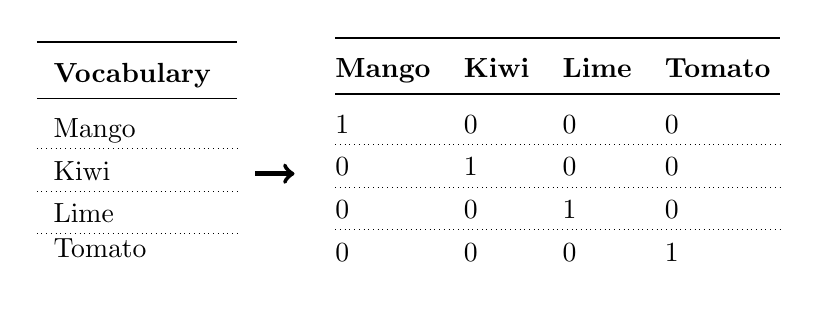
\begin{tikzpicture}
    \node (tab1) {%
        \begin{tabular}{l}\toprule
            \textbf{Vocabulary} \Tstrut\Bstrut\\\midrule
            Mango \Tstrut\Bstrut\\\hdashline
            Kiwi \Tstrut\Bstrut\\\hdashline
            Lime \Tstrut\Bstrut\\\hdashline
            Tomato
        \end{tabular}};

    \node [right=of tab1] (tab2) {%
        \begin{tabular}{@{}llll@{}}\toprule
              \textbf{Mango} & \textbf{Kiwi} & \textbf{Lime} & \textbf{Tomato} \Tstrut\Bstrut\\\midrule
              1 & 0 & 0 & 0 \Tstrut\Bstrut\\\hdashline
              0 & 1 & 0 & 0 \Tstrut\Bstrut\\\hdashline
              0 & 0 & 1 & 0 \Tstrut\Bstrut\\\hdashline
              0 & 0 & 0 & 1 \Tstrut\Bstrut
        \end{tabular}};
    \draw [ultra thick, transform canvas={yshift=-0.7em}, ->] (1.5,0) -- (2, 0);
    \end{tikzpicture}
    \caption{An example of one-hot encoded vectors. Each vector has a dimension for each distinct word of the vocabulary, and each component is a binary value.}
    \label{fig:one_hot_encoding}
\end{figure}

One-hot encodings are a popular choice when encoding categorical variables as they are fairly simple structures and can be constructed quickly and easily. However, their use is very impractical with large vocabularies, as the sparse representation demands large amounts of memory. For a vocabulary of size $n$, encoding all words has a space complexity of $\Theta(n^2)$. This makes it computationally infeasible to use on large datasets (where the vocabulary can easily exceed 100K words). Furthermore, one-hot vectors do not contain any inherent meaning---the construction of the one-hot vectors only depends on the position of words in the vocabulary. Swapping the order of two words in the vocabulary will change their one-hot vectors. This makes it impossible to reason about word meaning with one-hot vectors.

\inlineSection{Word Embeddings} We desire a scheme for encoding words into vectors that is both low-dimensional (space efficient) and which encodes meaning. One reasonable metric for a `good' encoding model is to say that words which are more similar should be closer together in the vector space. Notice how one-hot encoding does not satisfy this condition.\footnote{What does it even mean to take the distance or similarity between two one-hot vectors?}

A word embedding model, $\mathcal{W}$, is an $n$-dimensional real vector space, which maps words from a vocabulary, $V$, to an element of the vector space: $\mathcal{W}: V \rightarrow \mathbb{R}^n$. This vector space has the property that it \textit{encodes} rich semantic information. If well trained, one excellent consequence of word embeddings are that we can manipulating points in the vector space to reveal language features such as \textit{analogies} and \textit{word similarity}. For example, assume $\mathcal{W}$ is well-trained on the English language, then $\mathcal{W}(\text{king}) - \mathcal{W}(\text{man}) + \mathcal{W}(\text{woman}) \approx \mathcal{W}(\text{queen})$, where equality is measure of vector similarity.

Word2Vec is one approach to modelling words as dense vectors in a high-dimensional vector space introduced by Mikolov et. al. \cite{mikolov2013efficient}. In this way, we \textit{embed} words into a dense vector space. More specifically, we \textit{learn} these embeddings with a shallow neural-network, in the hopes that we these embeddings can approximate word similarity and reveal hidden relationships (such as analogies) between words.

\inlineSection{The Skip-Gram Model} There are multiple techniques for training a word2vec model; however, the general approach is to train the network to solve a language-related task on one-hot encoded words, and in the meantime let it learn an internal word embedding representation. Then, we simply extract the learned latent space to obtain our word embeddings. As a consequence, the choice for the task which our network `solves' is a critical decider of performance.

One approach which has proven to be very effective is the skip-gram architecture: a shallow neural-network trained to predict the context (or neighbourhood) of a target word \cite{goldberg2014word2vec, mikolov2013efficient}. The words in this neighbourhood are called \textit{context words} because the intuition is that neighbouring words are contextually meaningful.

Notice that while the skip-gram model is a supervised learning algorithm, we can generate training data in an unsupervised manner. Given some text document, $\mathcal{D}$, which represents a sequence of words, a sliding window of size $d$ is used to construct sample pairs. For some word at index $i$, at most $2d$ training samples are constructed by taking the following pairs of words:
\begin{equation*}
    (\mathcal{D}_{i}, \mathcal{D}_{i-d}), (\mathcal{D}_{i}, \mathcal{D}_{i-d+1}),\ldots, (\mathcal{D}_{i}, \mathcal{D}_{i+d}).
\end{equation*}
Figure \ref{fig:skipgram_sliding_window} illustrates how these target-context word pairs are constructed.

The skip-gram model consists of three layers: an input layer with $|V|$ neurons, a hidden layer with $N\leq|V|$ neurons, and an output layer with $|V|$ \cite{mikolov2013efficient}. The model takes in a one-hot encoded vector $\vec{X}$ as input and outputs a probability vector $\vec{Y}$ representing the probability distribution of the context over all words in the vocabulary. We use the softmax activation function to produce to normalize the outputs of the model to a probability distribution. The hidden layer contains a learned representation of the words. The weights of this layer, $\mat{W}^{|V|\times N}$, which we call the \textit{projection weights}, is a matrix representing the latent vector space containing our word embeddings: the $i$-th row of $\mat{W}$ gives the embedding vector of word $i$. Figure \ref{fig:skipgram_architecture} illustrates this architecture.

\begin{figure}[t]
    \centering
    \newcommand{\targetWordColour}{green!20!white}
    \newcommand{\contextWordColour}{orange!20!white}
    \renewcommand\tabularxcolumn[1]{m{#1}}
    \begin{tabularx}{0.5\textwidth}{>{\hsize=0.8\hsize}X>{\hsize=0.20\hsize}X@{}}\toprule
        \multicolumn{2}{c}{\textbf{Sample Construction via Sliding Window ($\bm{d=2}$)}}\\\midrule
        \textbf{Sentence} & \textbf{Contexts} \\\midrule
        \colorbox{\targetWordColour}{{[\targetWord{Sometimes}}}\colorbox{\contextWordColour}{{ we have]}} to fail to succeed. & we \newline have \\\hdashline
        \colorbox{\contextWordColour}{{[Sometimes}}\colorbox{\targetWordColour}{\targetWord{we}}\colorbox{\contextWordColour}{{have to]}} fail to succeed. & sometimes \newline have \newline to\\\hdashline
        \colorbox{\contextWordColour}{{[Sometimes we}}\colorbox{\targetWordColour}{\targetWord{have}}\colorbox{\contextWordColour}{{to fail]}} to succeed. & sometimes \newline we \newline to \newline fail\\\hdashline
        $\ldots$ & $\ldots$\\\hdashline
        Sometimes we have to \colorbox{\contextWordColour}{{[fail to}}\colorbox{\targetWordColour}{{\targetWord{succeed}]}}. &fail \newline to \newline\\\bottomrule
    \end{tabularx}
    \renewcommand\tabularxcolumn[1]{p{#1}}
    \caption{Example target-context pairs for the sentence, ``Sometimes we have to fail to succeed''. The radius of the sliding window is $2$ words.}
    \label{fig:skipgram_sliding_window}
\end{figure}

\inlineSection{Subsampling} The skip-gram approach of predicting the context word essentially boils down to a classification problem. In these sorts of problems, we want our data to be balanced so that it is representative of the true probability distribution. By generating training data using the sliding window approach, we oversample words which appear more often in the corpus. To remedy this, we use a technique proposed by Mikolov et. al. where we sample words according to a probability distribution designed to favour less frequently occurring words. This main advantage of subsampling is that we reduce the number of training examples, while maintaining the quality of the model. The sampling probability for a word $w\in V$ is given by
\begin{equation*}
    P(w)=\min\left\{\frac{t}{f(w)}\sqrt{\frac{f(w)}{t} + 1},1\right\},
\end{equation*}
where $f:V\rightarrow\Z$ gives the relative frequency of $w$ in the corpus \cite{mikolov2013efficient}.

\inlineSection{Training} We train the model with a process called \textit{stochastic gradient descent} (SGD). A computational approach to minimizing a function. Training consists of the following steps:
\begin{enumerate}
    \item Generate a target-context pair, $(w_t, w_c)$, mapping a target word, $w_t$, to one of its neighbours, $w_c$ (within a predefined window size).
    \item Forward propagate the one-hot vector representation of the input word, $w_t$, through the model.
    \item Calculate the training error according to a loss function, $\mathcal{L}$ (we use a variant of the cross entropy loss \cite{mikolov2013efficient, goldberg2014word2vec}).
    \item Perform propagation to compute the gradient of the loss function with respect to the weights.
    \item Update the weights: $\mat{W}_t=\mat{W}_{t-1}-\eta\nabla\mathcal{L}$, where $\mat{W}_t$ are the model weights at iteration $t$, $\mat{W}_{t-1}$ are the model weights in previous iteration, $\eta$ is the learning rate, and $\nabla\mathcal{L}$ are the gradients of the loss function. The learning rate is amount we should step in each iteration of SGD.
    \item Repeat steps 1 through 5 until we converge to a minimum.
\end{enumerate}

\inlineSection{Negative Sampling} When we train the skip-gram model, we have to update weights for each word in the vocabulary. For large datasets, this can be a very expensive operation. Negative sampling reduces the computation required for training by only updating $s$ words (which are \textit{not} a context of the target word; hence these are \textit{negative} examples). This means that we only update a small percentage of the model weights in each training iteration. Mikolov et. al. showed that for small datasets, $5\leq s\leq 20$ works best, whereas for large datasets, $2\leq s\leq 5$ suffice \cite{mikolov2013efficient}. In our experiments, we use $s=5$.

The negative samples are randomly sampled from the vocabulary with a probability distribution designed to favour more frequent words. The probability of selecting a word $w\in V$ as a negative sample is given by
\begin{equation}
    \label{eq:word2vec_neg_sample_distribution}
    P(w)=\frac{f(w)^\lambda}{\sum_{k=1}^{|V|}f(w_k)^\lambda},
\end{equation}
where $f$ is the relative frequency function and $\lambda$ is a hyper-parameter. In our experiments, we use $\lambda = 0.75$.

\inlineSection{Implementation} We implement the model using the TensorFlow deep learning library. We chose TensorFlow since it is a versatile library for training and deploying neural networks \cite{tensorflow2015-whitepaper}. It provides an interface for performing fast computation and linear algebra operations (such as matrix multiplication, which is core to training a neural work) on the GPU. It includes the \texttt{tf.keras} which simplifies the process of defining, training, and evaluating neural networks by providing implementations of common layers and activation functions such as 2D convolutional layers (\texttt{tf.keras.layers.Conv2D}), fully connected/linear layers (\texttt{tf.keras.layers.Dense}), the softmax activation function (\texttt{tf.keras.activations.softmax}), and more.

The \texttt{word2vec} modules provides a straightforward implementation of the architecture discussed in this section as a \texttt{tf.keras} subclass (see the \texttt{Word2Vec} class). To efficiently load the corpus, we leverage the the \texttt{tf.data} module. We use the \texttt{tf.data.Dataset} class to quickly load, tokenize, and batch our data (see the \texttt{make\_dataset} function).

\begin{figure*}[ht]
    \centering
    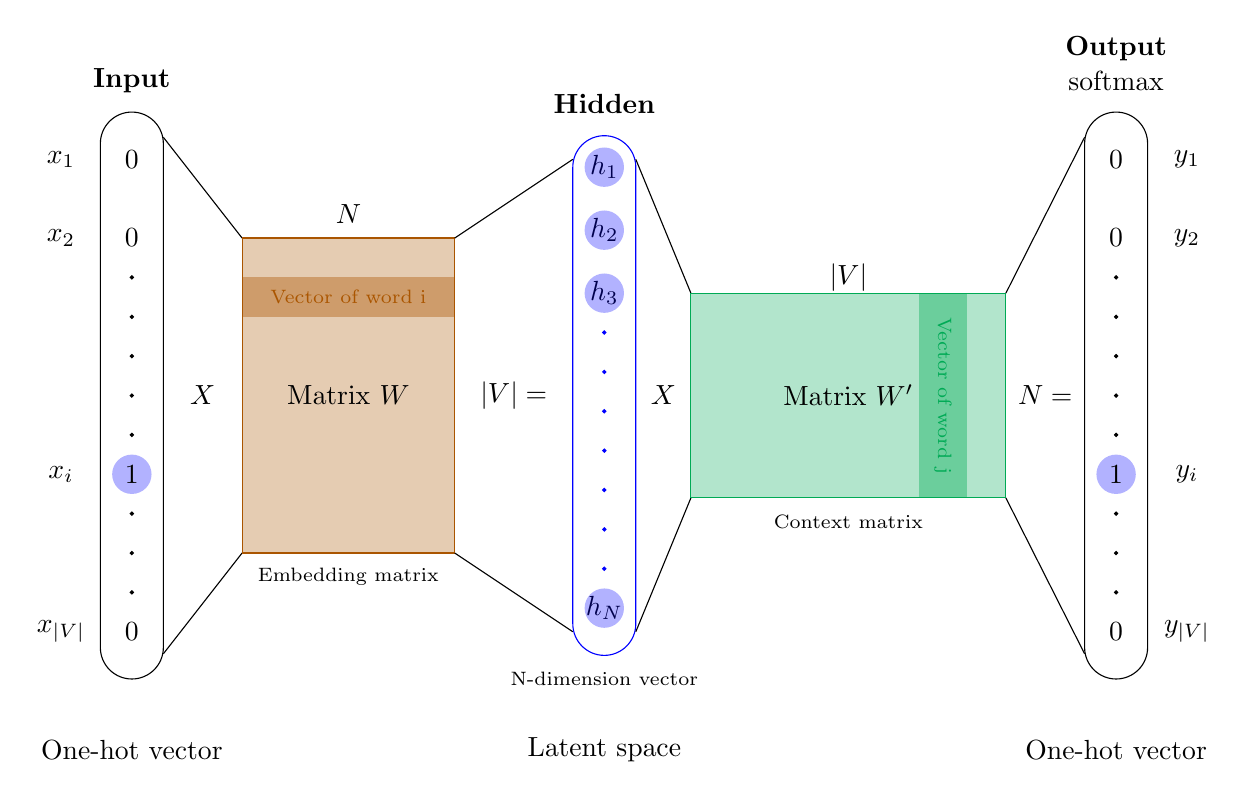
\begin{tikzpicture}
\node at (0.9, 8) {\bfseries Input};

\node at (0,7) {$x_1$};
\node at (0,6) {$x_2$};
\node at (0,3) {$x_i$};
\node at (0,1) {$x_{|V|}$};

\draw[rounded corners=0.4cm] (0.5,7.6) rectangle (1.3,0.4);

\node at (0.9,7) {0};
\node at (0.9,6) {0};
\filldraw (0.9,5.5) circle (0.02cm);
\filldraw (0.9,5) circle (0.02cm);
\filldraw (0.9,4.5) circle (0.02cm);
\filldraw (0.9,4) circle (0.02cm);
\filldraw (0.9,3.5) circle (0.02cm);
\fill[color=blue,opacity=0.3] (0.9,3) circle (0.25cm);
\node at (0.9,3) {1};
\filldraw (0.9,2.5) circle (0.02cm);
\filldraw (0.9,2) circle (0.02cm);
\filldraw (0.9,1.5) circle (0.02cm);
\node at (0.9,1) {0};

\draw (1.3,7.28) -- (2.3,6);
\draw (1.3,0.72) -- (2.3,2);

\node at (1.8,4) {$X$};

\filldraw[color={rgb:red,2;green,1},fill opacity=0.3] (2.3,6) rectangle (5,2);

\fill[color={rgb:red,2;green,1},fill opacity=0.4] (2.3,5.5) rectangle (5,5);
\node[color={rgb:red,2;green,1},font=\scriptsize] at (3.65,5.25) {Vector of word i};

\node at (3.65,6.3) {$N$};

\node at (3.65,4) {Matrix $W$};

\node[font=\scriptsize] at (3.65,1.7) {Embedding matrix};

\draw (5,6) -- (6.5,7);
\draw (5,2) -- (6.5,1);

\node at (5.75,4) {$|V| =$};

\node at (6.9, 7.7) {\bfseries Hidden};

\draw[rounded corners=0.4cm,color=blue] (6.5,7.3) rectangle (7.3,0.7);

\node at (6.9,6.9) {$h_1$};
\fill[color=blue,opacity=0.3] (6.9,6.9) circle (0.25cm);
\node at (6.9,6.1) {$h_2$};
\fill[color=blue,opacity=0.3] (6.9,6.1) circle (0.25cm);
\node at (6.9,5.3) {$h_3$};
\fill[color=blue,opacity=0.3] (6.9,5.3) circle (0.25cm);
\filldraw[color=blue] (6.9,4.8) circle (0.02cm);
\filldraw[color=blue] (6.9,4.3) circle (0.02cm);
\filldraw[color=blue] (6.9,3.8) circle (0.02cm);
\filldraw[color=blue] (6.9,3.3) circle (0.02cm);
\filldraw[color=blue] (6.9,2.8) circle (0.02cm);
\filldraw[color=blue] (6.9,2.3) circle (0.02cm);
\filldraw[color=blue] (6.9,1.8) circle (0.02cm);
\node at (6.9,1.3) {$h_N$};
\fill[color=blue,opacity=0.3] (6.9,1.3) circle (0.25cm);

\node[font=\scriptsize] at (6.9,0.4) {N-dimension vector};

\draw (7.3,7) -- (8,5.3);
\draw (7.3,1) -- (8,2.7);

\node at (7.65,4) {$X$};

\filldraw[color={rgb:green,2;blue,1},fill opacity=0.3] (8,5.3) rectangle (12,2.7);

\fill[color={rgb:green,2;blue,1},fill opacity=0.4] (10.9,5.3) rectangle (11.5,2.7);
\node[color={rgb:green,2;blue,1},rotate=270,font=\scriptsize] at (11.2,4) {Vector of word j};

\node at (10,5.5) {$|V|$};

\node at (10,4) {Matrix $W'$};

\node[font=\scriptsize] at (10,2.4) {Context matrix};

\draw (12,5.3) -- (13,7.28);
\draw (12,2.7) -- (13,0.72);

\node at (12.5,4) {$N =$};

\draw[rounded corners=0.4cm] (13,7.6) rectangle (13.8,0.4);

\node at (13.4,7) {0};
\node at (13.4,6) {0};
\filldraw (13.4,5.5) circle (0.02cm);
\filldraw (13.4,5) circle (0.02cm);
\filldraw (13.4,4.5) circle (0.02cm);
\filldraw (13.4,4) circle (0.02cm);
\filldraw (13.4,3.5) circle (0.02cm);
\fill[color=blue,opacity=0.3] (13.4,3) circle (0.25cm);
\node at (13.4,3) {1};
\filldraw (13.4,2.5) circle (0.02cm);
\filldraw (13.4,2) circle (0.02cm);
\filldraw (13.4,1.5) circle (0.02cm);
\node at (13.4,1) {0};

\node at (13.4, 8.4) {\bfseries Output};
\node at (13.4, 8) {softmax};

\node at (14.3,7) {$y_1$};
\node at (14.3,6) {$y_2$};
\node at (14.3,3) {$y_i$};
\node at (14.3,1) {$y_{|V|}$};

\node at (0.9,-0.5) {One-hot vector};
\node at (6.9,-0.5) {Latent space};
\node at (13.4,-0.5) {One-hot vector};
\end{tikzpicture}
    \caption{The architecture of the skip-gram model. Figure inspired by Weng \cite{weng_learning_embeddings}.}
    \label{fig:skipgram_architecture}
\end{figure*}

\subsection{Sentiment Classification}
In the last few years, transformer models have been shown to be widely effective on a variety of tasks in natural language processing. They have ushered in a new interest in applying transfer learning in natural language. In \textit{Language Models are Few-shot Learners}, Brown et. al. showed that a massively scaled up stack of transformer-decoder layers consisting of 175 billion parameters (GPT-3) could achieve strong performance on many NLP tasks without any further model training.

\inlineSection{BERT \& Transfer Learning} The Bidirectional Encoder Representations from Transformer, or BERT for short is a similar general-purpose transformer model designed for transfer learning applications. The model is pre-trained to learn deep representations of text in an unsupervised manner. Then, the pre-trained model can be fine-tuned on a NLP tasks by simply adding a new output layer. Devlin et. al. showed that this approach can achieve state-of-the-art performance on various NLP tasks (such as question answering and language inference) \cite{devlin2019bert}.

Much of the state-of-the-art performance of these models comes from the their main ingredient: the transformer \cite{vaswani2017attention}. Using an attention mechanism, transformers are able to model long-term dependencies in the data. At each training step, the attention mechanism allows the transformer to focus on a specific part of the input. In this way, attention is focus, which mimicks the natural way which we process information. The second ingredient in the success of these models is their size. By stacking many transformers on top one another, we are able to increase the models capacity; however, this comes at a computational cost.

Transfer learning enables us to solve complex problems in natural language processing without a large dataset or the computational requirements of training a full-scale GPT or BERT model. For this reason, we use a pre-trained BERT model and then fine-tune it on the climate change sentiment dataset (see Section \ref{sec:datasets}). Figure \ref{fig:bert_architecture} illustrates the architecture of the classification model.

\begin{figure}[ht]
    \centering
    \definecolor{classifierText}{HTML}{52575F}
\definecolor{bertBg}{HTML}{FFF5B5}
\begin{tikzpicture}[scale=0.6, every node/.style={scale=0.6}]
\node[font=\Large,anchor=west] at (-0.5,4) {\bfseries Dataset:};

% A
\filldraw[fill=green,draw=gray,fill opacity=0.3] (3,5) rectangle (10,4);
\node at (6.5,4.5) {Smh. `Global warming'...it's $-20^\circ$ C.};

\filldraw[fill=purple,draw=gray,fill opacity=0.3] (10,5) rectangle (12,4);
\node at (11,4.5) {-1};

% B
\filldraw[fill=green,draw=gray,fill opacity=0.3] (3,4) rectangle (10,3);
\node at (6.5,3.5) {Maybe you are not so clever.};

\filldraw[fill=purple,draw=gray,fill opacity=0.3] (10,4) rectangle (12,3);
\node at (11,3.5) {0};

\filldraw[fill=green,draw=gray,fill opacity=0.3] (3,3) rectangle (10,2);
\node at (6.5,2.5) {join me! \#climatestrike};

\filldraw[fill=purple,draw=gray,fill opacity=0.3] (10,3) rectangle (12,2);
\node at (11,2.5) {1};

\node[color=green!60!black] at (6.5,5.5) {Tweet};

\node[color=purple!60!black] at (11,5.5) {Class};

\node[font=\Large,anchor=west,text width=3cm] at (-0.5,9) {\textbf{Pre-trained}};

\filldraw[rounded corners=0.4cm,fill=bertBg,draw=black!70!white,line width=0.08cm] (3,11) rectangle (12,7);
\draw[thick, opacity=0.5] (8,7.5) -- (12,7.5);
\fill[color=white, opacity=0.8] (9.3,9.7) circle (0.6cm);
\fill[color=white, opacity=0.8] (10.7,9.7) circle (0.6cm);
\fill[color=brown, opacity=0.8] (9.4,9.7) circle (0.25cm);
\fill[color=brown, opacity=0.8] (10.6,9.7) circle (0.25cm);
\draw[line width=0.3cm, opacity=0.5] (8.3,10.5) -- (10,10.2);
\draw[line width=0.3cm, opacity=0.5] (10,10.2) -- (11.7,10.5);
\fill[color=orange, opacity=0.5] (10,8.5) ellipse (0.7cm and 1cm);
% \node at (10,8.5) {BERT};
\node[opacity=0.8] at (4.7,9.9) {\Huge \textsf{\textbf{BERT}}};

\filldraw[rounded corners=0.2cm,color=classifierText,fill=blue!10!white,line width=0.08cm] (3,14.5) rectangle (7,12.5);
\node[font=\Large] at (5,13.5) {\textcolor{classifierText}{\textsf{\textbf{Classifier}}}};

\draw[->,line width=0.08cm] (5,11) -- (5,12.5);

% Stuff
\filldraw[fill=red!40!white,draw=gray] (8.5,15) rectangle (10,14);
\node at (9.25,14.5) {91\%};

\filldraw[fill=red!20!white,draw=gray] (8.5,14) rectangle (10,13);
\node at (9.25,13.5) {5\%};

\filldraw[fill=red!10!white,draw=gray] (8.5,13) rectangle (10,12);
\node at (9.25,12.5) {4\%};

\node[anchor=west] at (10.2,14.5) {Positive};
\node[anchor=west] at (10.2,13.5) {Neutral};
\node[anchor=west] at (10.2,12.5) {Negative};

\draw[->,line width=0.08cm] (7,13.5) -- (8.5,13.5);
\end{tikzpicture}
    \caption{The architecture of the classification model. It uses a pre-trained BERT backbone with a fully-connected classification head with softmax activation. Figure inspired by Alammar \cite{illustrated_bert}.}
    \label{fig:bert_architecture}
\end{figure}

\inlineSection{Training} The pre-trained BERT model checkpoints are provided by TensorFlow via TF Hub, a framework for performing transfer learning with TensorFlow \cite{tf_hubs}. We use the \texttt{tensorflow\_hub} package to download and load the model, and then append a \texttt{tf.keras.layers.Dense} layer to the output of the BERT model to obtain our classification model \cite{tf_keras_docs, tf_hubs_github}. The model is trained to minimise the cross entropy loss (we use the \texttt{tf.keras.losses.SparseCategoricalCrossentropy} implementation), using the AdamW optimizer (from the \texttt{official.nlp.optimization} package) \cite{tf_officials_github}. This is all contained within the \texttt{train\_text\_classifier.py} script.

\inlineSection{Interpreting Sentiment} Our sentiment classification models predicts a probability distribution over all sentiment classes (i.e. positive, negative, and neutral). But, how can we produce a single sentiment value for an input? One approach is to take the class with the largest probability; however, what happens if two classes have similar probabilities? What if they differ by a very small factor? In this case, resolving the distribution to its maximum value might not accurately reflect the true class of the input. We address this problem by \textit{sampling} from the probability distribution. If $\hat{\vec{P}}$ is a probability vector representing the predicted probability distribution for $m$ classes labelled $\{1,2,\ldots,m\}$, then for some $1\leq i \leq m$, the probability of sampling class $i$ is given by $\hat{\vec{P}}_i$.

% \subsection{False News Detection}

\subsection{Embedding Projection}
The ability to explore high-dimensional vector spaces such as word embeddings is crucial both in the development of models, and in the research of new techniques. Neural networks, embeddings, and other forms of highly-parameterised models are often referred to as `black boxes' because studying the structure of these models is extremely difficult and sometimes impossible. At the same time, the ability to `peek' into the internals is key in testing and debugging models. For example, we might want to verify that an embedding space is truly representing the desired features.

Compared to `conventional' data, understanding word embeddings can be particularly challenging due to the high-dimensionality of the data. The sheer number of dimensions in the embedding space makes it impractical to work with the raw vectors. Similarly, conventional visualisation tools are seldom useful due to both a lack of support for large dimensional data, and a lack of interactivity which is key for navigating a dense vector space such as word embeddings. We follow an approach by Smilkov et. al. where we reduce the dimensional of the embedding vectors to project it into a vector space which is human-friendly and easy to visualise \cite{smilkov2016embedding}. In this section, we present an interactive visualisation and analysis tool for \textit{projecting} high-dimensional vector spaces, such as word embeddings, into two- or three-dimensional space

\inlineSection{Overview} The embedding projector is a Python application that can be ran from the command-line (see the \texttt{embedding\_projector.py} module) built using the Plotly Dash framework \cite{plotly}. Figure \ref{fig:embedding_projector} shows the interface of the embedding projector. The application allows users to explore an arbitrary vector space given an embedding matrix; however, it is mostly tailored for use with word embeddings. The embedding projector allows the user to not only inspect the projected vector space, but also to search for words (in the analysis panel) and isolate the neighbouring points of a given selection (i.e. view a scatter plot only containing the neighbours).

\begin{figure*}[ht]
    \centering
    \begin{tikzpicture}[
        x=1mm, y=1mm,
    ]
    \node[anchor=south west=inner sep=0pt] (fig1) at (0, 0) {\fbox{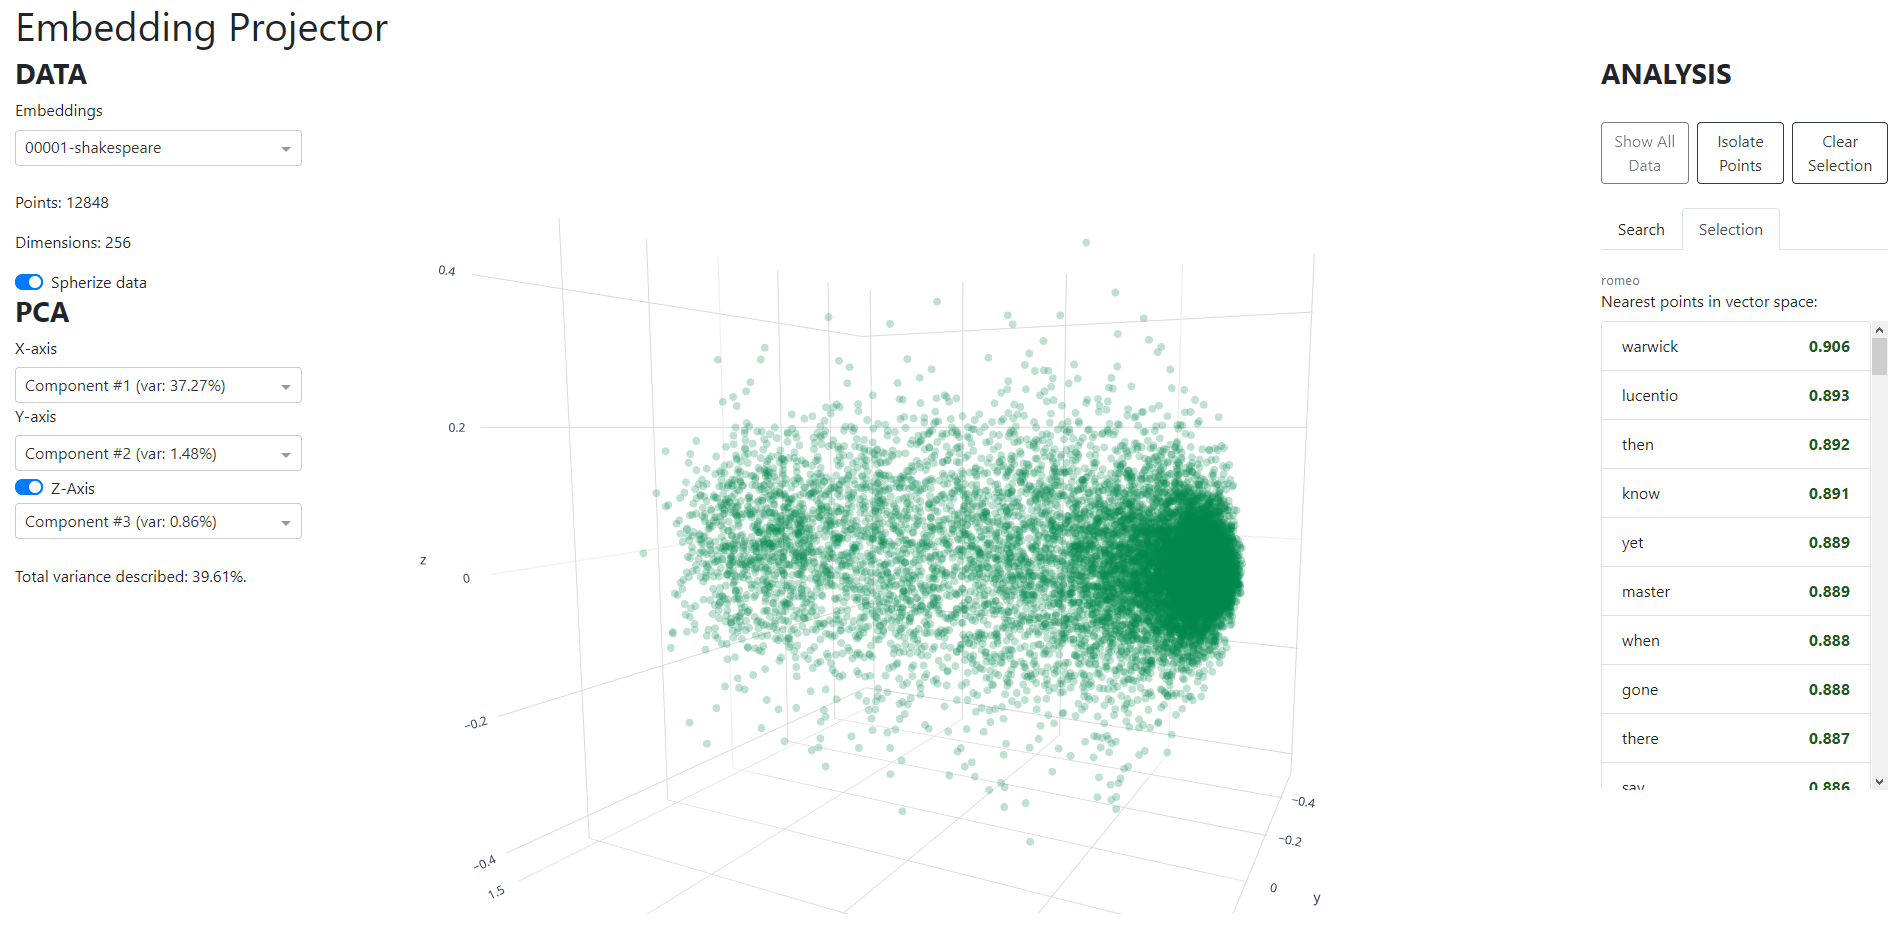
\includegraphics[width=0.8\textwidth]{EmbeddingProjector.png}}};

    % Data panel
    \filldraw[draw=red!50!white,fill=red,fill opacity=0.05] (2.3,70) rectangle (27,54);

    \filldraw[draw=red!50!white,fill=red!20!white,] (27-5, 70) rectangle (27,70-5) node[color=black,opacity=1,pos=0.5] {1};

    % PCA
    \filldraw[draw=red!50!white,fill=red,fill opacity=0.05] (2.3,52) rectangle (27,28);

    \filldraw[draw=red!50!white,fill=red!20!white,] (27-5, 52) rectangle (27,52-5) node[color=black,opacity=1,pos=0.5] {2};

    % Scatter plot view
    \filldraw[draw=red!50!white,fill=red,fill opacity=0.05] (2.3+50,45) rectangle (27+70,18);

    \filldraw[draw=red!50!white,fill=red!20!white,] (2.3+50, 45) rectangle (2.3+50+5,45-5) node[color=black,opacity=1,pos=0.5] {3};

    % Analysis panel
    \filldraw[draw=red!50!white,fill=red,fill opacity=0.05] (2.3+121,70) rectangle (27+121,10);

    \filldraw[draw=red!50!white,fill=red!20!white,] (27+121-5, 70) rectangle (27+121,70-5) node[color=black,opacity=1,pos=0.5] {4};

    \end{tikzpicture}
    \caption{The interface of the embedding projector: (1) the data panel, (2) the PCA panel, where users can choose any combination of two or three principle components, (3) the view of the projected data, and (4) the analysis panel, where users can search for words and explore their neighbours in the embedding space.}
    \label{fig:embedding_projector}
\end{figure*}

\inlineSection{Principle Component Analysis} To visualise the high-dimensional embedding vectors, we need to reduce it to a space that can be easily understood by a human: two- or three-dimensions. We use Principle Component Analysis (PCA), a common dimension reductionality approach to achieve this. For a given embedding matrix, we first compute the top ten principle components (these are the components with the most explained variance). Then, we select the top three of those components as our choice for the $x$, $y$, and $z$ dimensions of the projected space. While this means that the projected view is not an exact representation of the embedding geometry, it provides a very good approximation to the density of the space, which makes it ideal for analysing similarity and closeness of data points. The PCA panel (see Figure \ref{fig:embedding_projector}) allows users to configure which principle components correspond to which axis. We use the \texttt{sklearn.decomposition.PCA} implementation which supports two algorithms for computing the principle components: taking the eigenvalues of the covariance matrix, or performing singular value decomposition (the algorithm for computing the PCA is chosen automatically) \cite{scikit-learn}.

\inlineSection{Suffix Trees} Searching the embedding space is crucial for adequate exploration of the data. For word embeddings, this means that we must be able to search for words in the vocabulary and find their corresponding embedding vector in the projected space. We say that a word $w\in V$ is a search result if the query, $q$, is a substring of $w$.

A naive algorithm would iterate through the whole vocabulary, and check each word against the query. Of course, this is incredibly inefficient. For each query, we have to check against the \textit{whole} vocabulary. Instead, we use suffix trees to efficiently perform substring searching on the vocabulary. This reduces the running time to $\mathcal{O}(|q|)$, at the cost of an initial startup of $\mathcal{O}(|V|)$, where $|q|$ is the length of the query. For large vocabularies (such as the ones we train in this paper), this has a substantial performance difference.

We use a suffix tree implementation provided by the \texttt{suffix\_trees} package \cite{suffix_trees_package}. Since suffix trees operate on a single string input, we convert our vocabulary into a space-separated string, and then feed that to the suffix tree. Queries on this suffix trees gives us a set of indices indicating where in the string the queried substring occurs. To resolve these matches into words, we exploit the structure of the string that the suffix tree was built on: the fact that it is space-separated. Thus, for each index, we search for the first space to the left and right of the match to determine the word. This has a runtime of $\mathcal{O}(L)$, where $L$ is the length of the largest word in the vocabulary. Considering the fact that the length word in the English language is only 45 characters, and word frequency substantially decreases with length, this is not a bottleneck \cite{wiki:longest_words, smith2012distinct}.

\inlineSection{$\bm{K}$-Nearest Neighbour Search} We use a $K$-nearest neighbours model to efficiently find the most similar word embeddings. A naive `bruteforce' algorithm to find the top $k$ similar vectors would have to iterate through the whole vocabulary, compute the pairwise cosine similarity, and then sort the results, for a total running time of $\Theta(|V|\times Nk)$. In comparison, a $k$-nearest neighbours implemented as a KD-tree has a query runtime of $\Theta(k\log{|V|})$, which is a vast improvement from the naive algorithm. This comes with a startup cost of $\Theta(|V|\times N)$, but it is negligble in the long-run. And the model implemented as a Ball tree has a similar run-time. We use the \texttt{sklearn.neighbors.KNeighborsClassifier} implementation which supports both KD-trees and Ball trees (automatically chosen based on the type of data) \cite{scikit-learn}.

\subsection{\textit{K}-Hop Graphs: Visualising Word Relation}

To perform an accurate analysis of tweet content, we must understand how words are used with one another, and in which contexts. Leveraging our word2vec models, we visualise the relationship between similar words as a graph, following the technique used by Schild et. al.

\inlineSection{Infinity-Hop Graph}
A $\infty$-hop graph is an undirected weighted graph whose nodes are words. It models the relationship between every word in the vocabulary. We say that for some distinct $w_1,w_2\in V$, an edge with weight $S(w_1,w_2)$, between $w_1$ and $w_2$ exists if and only if $S(w_1,w_2)\geq\alpha$, where $S$ is an arbitrary similarity metric between two words and $\alpha$ is a similarity threshold.

In this paper, we define $S$ as the \textit{cosine similarity} between the two word embedding vectors for words $w_1$ and $w_2$. Geometrically, this similarity metric can be interpreted as the cosine of the angle between the two vectors.

\inlineSection{$\bm{K}$-Hop Graphs} We say that the $k$-hop graph for some word of interest, $T\in V$, is a subgraph of the $\infty$-hop graph, consisting of all the nodes and their respective edges in the $\infty$-hop graph that are at most $k$ edges from $T$. Informally, this means that the $k$-hop graph is the $\infty$-hop graph limited to at most $k$ `hops' from a word of interest.

Formally, the $k$-hop graph, $\mathcal{H}_k^{(T)}$, for a vocabulary $V$, word of interest $T\in V$, similarity function $S:V^2\rightarrow\R$, and similarity threshold $\alpha\in\R$, is a subgraph of the $\infty$-hop graph defined by the ordered pair
\begin{equation*}
    \mathcal{H}_k^{(T)}=\left(N_k^{(T)}, E_k^{(T)}\right),
\end{equation*}
where $N_k^{(T)}\subseteq N_\infty$ is the node or vertex set, and $E_k^{(T)}\subseteq E_\infty$ is the edge set, where $N_\infty$ and $E_\infty$ are the node and edge sets for the $\infty$-hop graph respectively.

For all $w\in N_\infty$, the word $w$ is a node of the $k$-hop graph if and only if there exists a path with at most $k$ edges from $w$ to $T$ in the $\infty$-hop graph. The edges of $\mathcal{H}_k^{(T)}$ are simply those which are leftover after filtering out nodes which are not reachable from $T$ in at most $k$ edges. So,
\begin{equation*}
    E_k^{(T)}=\left\{(w_1,w_2)\in  E_\infty \mid w_1,w_2\in N_k^{(T)} \right\}.
\end{equation*}

\inlineSection{Visualising the Graph}  We employ several algorithms for visualising the $k$-hop graphs. To build, process, and manipulate the graphs, we use the NetworkX Python package---a popular library for studying graphs and networks \cite{networkx_docs}. After computing the node and edge set of the $k$-hop graph, we use a force-directed layout algorithm called ForceAtlas2 (using the \texttt{fa2} package) to spatilize the network \cite{Jacomy2014, fa2_networkx}. The algorithm takes into account edge weights to determine an optimal graph layout. Then, we perform Louvain  community detection (using the \texttt{python-louvain} package) to extract communities from the network in an unsupervised manner \cite{python_louvain, Blondel_2008}. We assign a colour to each community, and colour each node with that colour. Edges colours are determined by the colour of the source node.

\inlineSection{Implementation Details} Building the infinity-hop graph for the projection weights matrix, $\mat{W}^{|V|\times N}$ (where $|V|$ is the vocabulary size and $N$ is the embedding dimensionality) requires the computation of a pairwise cosine similarity matrix, $\mat{M}$. For large vocabularies, computing $\mat{M}$ is a particularly expensive operation, since it requires $\Theta(|V|^2)$ space. For a matrix with 32-bit floating-point values (\texttt{float32}), this can easily exceed 40 GB ($|V|\geq 100,000$).

However, notice that we don't actually need to store anything: building the infinity-hop graph simply requires that we keep the pairs whose similarity is above a threshold. So, we reduce the memory footprint by \textit{batching} the computations. For some batch size $B\in\N$, we iteratively construct the infinity-hop graph by computing the pairwise cosine similarity matrix between $\mat{W}$ and $B$ rows of $\mat{W}$ at a time. More specifically, for some row offset $i\leq \left\lfloor\frac{|V|}{B}\right\rfloor + 1$, we compute the pairwise cosine similarity matrix, $\mat{M}^\prime$ as the normalized dot product of a smaller matrix and $\mat{W}$, given by
\begin{equation*}
    \mat{M}^\prime=\frac{\langle\mat{C}^{(i)}, \mat{W}\rangle}{\|\mat{C}^{(i)}\|_2\|\mat{W}\|_2},
\end{equation*}
where $\mat{C}^{(i)}$ is a matrix containing all rows of $\mat{W}$ with indices between $iB$ and $(i+1)B$. Then, we apply filtering on $\mat{M}^\prime$ to build the infinity-hop graph. Converting rows from `local' indices to their word embedding index just requires adding the row offset. For example, the first row of $\mat{M}^\prime$ corresponds to the $B$-th row of $\mat{W}$, and in general the $j$-th row of $\mat{M}^\prime$ is the $j+Bi$-th row of $\mat{W}$, where $i$ is the row offset.

This approach yields a space complexity of $\Theta(|V|\times B)$. For $B=256$ and $|V|=100,000$, this means that we only need roughly 102 MB of available RAM---a significant reduction from the 40 GB requirement of the previous algorithm.

\subsection{Instructions for Reproducibility}
We provide the source code for running all experiments, along with the training and testing data, and pre-trained model weights.\footnote{https://github.com/GalacticGlum/csc110-course-project}.

\inlineSection{Note About Requirements} Some of the required packages include native code. Unfortunately, these libraries do not come with pre-compiled binaries for Python 3.8 so a C/C++ compiler is required to build them from source when installing requirements. On Windows, download \textcolor{blue}{\href{https://visualstudio.microsoft.com/downloads/\#build-tools-for-visual-studio-2019}{MSVC 1.14+}}. On Mac or Linux, \texttt{gcc} or \texttt{g++} will work.

\inlineSection{Dataset} Click \href{https://drive.google.com/file/d/16TWeFHXcywSoc13vrsw9SxEZ4lJndp4g/view?usp=sharing}{\textcolor{blue}{here}} to download the data used to train and evaluate the models. Note that this is a fairly large file (roughly 4 GB compressed), so downloading may take a while depending on internet connection. Extract the archive in a folder called \texttt{data} (under the root project directory).

\inlineSection{Model Weights} Click \href{https://mega.nz/file/b0EViYzT\#MEgk2yE5M3fjYUimtyhAj6XzZK5lZr7G29bPGN1rc20}{\textcolor{blue}{here}} to download the \textbf{full} model checkpoints and weights. Note that this is a fairly large file (roughly 20 GB compressed), so downloading may take a while depending on the internet connection.

For this reason, we also provide a subset of the trained model weights (roughly 1 GB compressed), which contain the word embeddings for tweets posted in April, May, and June, 2020 along with the trained sentiment classification model. We also provide light-weight word embeddings (roughly 50 MB) for a corpus consisting of Shakespeare's works which were used for testing the models and visualisation tools.

Click \href{https://mega.nz/file/28FQmbZY\#nHoAVB3AL0OdyyP58KVLjMG6GTm5eLt77EgyF60xOn4}{\textcolor{blue}{here}} to download a \textbf{subset} of the model checkpoints and weights. In the interest of space, we omit all checkpoints except for the latest one. Furthermore, for the word2vec models, since the output layer is not used outside of training, we omit the checkpoints entirely. Instead, we only provide the projection weights (\texttt{proj\_weights.npy}), model vocabulary (\texttt{vocab.txt}), and tokenizer state (\texttt{tokenizer.json}).

After the download is complete, extract the archive in the root project directory. The zip file already contains an \texttt{output} sub directory, so there is no need to create one.

\inlineSection{Running the Experiments \& Visualisations} See the provided \texttt{main.py} for starter code to run the embedding projector, and/or generate a $k$-hop graph.

\section{Results}\label{sec:results}
\begin{table*}[h]
    \centering
    \begin{tabularx}{\textwidth}{>{\hsize=0.1\hsize}X>{\hsize=0.30\hsize}XX@{}}\toprule
        \multicolumn{3}{c}{\textbf{Major Events}}\\\midrule
        \textbf{\#} & \textbf{Day} & \textbf{Event}\\\midrule
        1 & June 8, 2018 & The 44th G7 summit is held in Canada. Donald Trump gets into multiple disputes with other world leaders: insults Japanese Prime Minsiter Shinzo Abe, and speaks harshly about Canadian Prime Minister Justin Trudeau \cite{wiki:g7_44}.\\\hdashline
        2 & September 14, 2018 & Global Climate Action Summit is held \cite{un_climate_action_summit}.\Tstrut\Bstrut\\\hdashline
        3 & August 19, 2019 & NASA Confirms the uptick in Amazon rainforest fire activity \Tstrut\Bstrut\\\hdashline
        4 & March 15, 2019 & A series of global school strikes. The first organised by Greta Thunberg. Over 1.4M people participate. \cite{wiki:greta_climate_strikes}. \Tstrut\Bstrut\\\hdashline
        5 & September 20, 2019 & Global week of climate action. Over 4M people participate. \cite{wiki:greta_climate_strikes}.\Tstrut\Bstrut\\\hdashline
        6 & November 4, 2019 & The Trump administration gives a formal notice of intention to withdraw from the Paris Agreement \cite{wiki:us_leaves_paris_agreement}.\Tstrut\Bstrut\\\hdashline
        7 & June 12, 2020 & The 46th G7 summit is cancelled due to COVID-19 \cite{wiki:g7_46}.\\\bottomrule
    \end{tabularx}
    \caption{Major climate events. Figures \ref{fig:monthly_mentions_ClimateChange_GlobalWarming}-\ref{fig:monthly_mentions_ClimateKeyFigures} are annotated with these events.}
    \label{tab:major_events}
\end{table*}

\subsection{Temporal Analysis}
% FIGURE FOR MONTHLY MENTIONS OF CLIMATE CHANGE/GLOBAL WARMING
\definecolor{eventColour}{HTML}{27b898}
\newcommand{\eventAnnotationsFreq}{
    \draw [color=eventColour,dashed, ultra thick] (2018-6-8,0) -- (2018-6-8,10000);
    \draw [color=eventColour,dashed, ultra thick] (2018-9-14,0) -- (2018-9-14,10000);
    \draw [color=eventColour,dashed, ultra thick] (2019-8-19,0) -- (2019-8-19,10000);
    \draw [color=eventColour,dashed, ultra thick] (2019-9-20,0) -- (2019-9-20,10000);
    \draw [color=eventColour,dashed, ultra thick] (2019-11-4,0) -- (2019-11-4,10000);
    \draw [color=eventColour,dashed, ultra thick] (2020-6-12,0) -- (2020-6-12,10000);
}

\newcommand{\eventAnnotationsProp}{
    \draw [color=eventColour,dashed, ultra thick] (2018-6-8,0) -- (2018-6-8,0.001);
    \draw [color=eventColour,dashed, ultra thick] (2018-9-14,0) -- (2018-9-14,0.001);
    \draw [color=eventColour,dashed, ultra thick] (2019-8-19,0) -- (2019-8-19,0.001);
    \draw [color=eventColour,dashed, ultra thick] (2019-9-20,0) -- (2019-9-20,0.001);
    \draw [color=eventColour,dashed, ultra thick] (2019-11-4,0) -- (2019-11-4,0.001);
    \draw [color=eventColour,dashed, ultra thick] (2020-6-12,0) -- (2020-6-12,0.001);
}

\begin{figure*}[!hpb]
    \centering
    \begin{subfigure}{0.45\textwidth}
        \centering
        \begin{tikzpicture}
        \pgfplotsset{compat=1.12}
            \begin{axis}[
                title={Frequency},
                align=center,
                date coordinates in=x,
                % xtick=data,
                xticklabel style=
            		{rotate=60, anchor=east, yshift=-10pt},
                xticklabel={\year.\month},
                date ZERO=2009-08-18,% <- improves precision!
                max space between ticks=100pt,
                try min ticks=10,
                legend pos=north west,
                ylabel={Frequency},
                grid=major
            ]
            \addplot+ [thick, mark=none] table {\WordClimateChangeFrequency};
            \addplot+ [ultra thick, mark=none, dashed] table {\WordGlobalWarmingFrequency};
            \addlegendentry{climate change}
            \addlegendentry{global warming}
            \eventAnnotationsFreq
            \end{axis}
        \end{tikzpicture}
    \end{subfigure}
    \hfill
    \begin{subfigure}{0.45\textwidth}
        \centering
        \begin{tikzpicture}
        \pgfplotsset{compat=1.12}
            \begin{axis}[
                title={Proportion},
                align=center,
                date coordinates in=x,
                % xtick=data,
                xticklabel style=
            		{rotate=60, anchor=east, yshift=-10pt},
                xticklabel={\year.\month},
                date ZERO=2009-08-18,% <- improves precision!
                max space between ticks=100pt,
                try min ticks=10,
                legend pos=north west,
                ylabel={Proportion},
                grid=major
            ]
            \addplot+ [thick, mark=none] table {\WordClimateChangeProportion};
            \addplot+ [ultra thick, mark=none, dashed] table {\WordGlobalWarmingProportion};
            \addlegendentry{climate change}
            \addlegendentry{global warming}
            \eventAnnotationsProp
            \end{axis}
        \end{tikzpicture}
    \end{subfigure}
    
    \caption{Monthly mentions of the terms ``climate change'' and ``global warming'' on Twitter.}
    \label{fig:monthly_mentions_ClimateChange_GlobalWarming}
\end{figure*}

% FIGURE FOR MONTHLY MENTIONS FOR CLIMATE ACTIVISM KEYWORDS
\begin{figure*}[!hpb]
    \centering
    \begin{subfigure}{0.45\textwidth}
        \centering
        \begin{tikzpicture}
        \pgfplotsset{compat=1.12}
            \begin{axis}[
                title={Frequency},
                align=center,
                date coordinates in=x,
                % xtick=data,
                xticklabel style=
            		{rotate=60, anchor=east, yshift=-10pt},
                xticklabel={\year.\month},
                date ZERO=2009-08-18,% <- improves precision!
                max space between ticks=100pt,
                try min ticks=10,
                legend pos=north west,
                ylabel={Frequency},
                grid=major
            ]
            \addplot [color=blue, mark=none] table {\WordClimateStrikeFrequency};
            \addplot [mark=none, color=red] table {\WordClimateCrisisFrequency};
            \addplot [mark=none, color=orange] table {\WordClimateJusticeFrequency};
            \addplot [mark=none, color=black] table {\WordClimateActivistsFrequency};
            \addplot [mark=none, color=purple] table {\WordClimateActivistFrequency};
            \addplot [mark=none, color=green!50!black] table {\WordClimateActionFrequency};
            \addlegendentry{climate strike}
            \addlegendentry{climate crisis}
            \addlegendentry{climate justice}
            \addlegendentry{climate activists}
            \addlegendentry{climate activist}
            \addlegendentry{climate action}
            \eventAnnotationsFreq
            \end{axis}
        \end{tikzpicture}
    \end{subfigure}
    \hfill
    \begin{subfigure}{0.45\textwidth}
        \centering
        \begin{tikzpicture}
        \pgfplotsset{compat=1.12}
            \begin{axis}[
                title={Proportion},
                align=center,
                date coordinates in=x,
                % xtick=data,
                xticklabel style=
            		{rotate=60, anchor=east, yshift=-10pt},
                xticklabel={\year.\month},
                date ZERO=2009-08-18,% <- improves precision!
                max space between ticks=100pt,
                try min ticks=10,
                legend pos=north west,
                ylabel={Proportion},
                grid=major
            ]
            \addplot+ [color=blue, mark=none] table {\WordClimateStrikeProportion};
            \addplot+ [color=red, mark=none, color=red] table {\WordClimateCrisisProportion};
            \addplot+ [color=orange, mark=none, color=orange] table {\WordClimateJusticeProportion};
            \addplot+ [color=black, mark=none] table {\WordClimateActivistsProportion};
            \addplot+ [color=purple, mark=none] table {\WordClimateActivistProportion};
            \addplot+ [color=green!50!black, mark=none] table {\WordClimateActionProportion};
            \addlegendentry{climate strike}
            \addlegendentry{climate crisis}
            \addlegendentry{climate justice}
            \addlegendentry{climate activists}
            \addlegendentry{climate activist}
            \addlegendentry{climate action}
            \eventAnnotationsProp
            \end{axis}
        \end{tikzpicture}
    \end{subfigure}
    \caption{Monthly mentions of the terms ``climate strike'', ``climate justice'', and``climate activists'', ``climate activist'', and ``climate action'' on Twitter.}
    \label{fig:monthly_mentions_ClimateActivism}
\end{figure*}

% FIGURE FOR MONTHLY MENTIONS FOR CLIMATE CHANGE SKEPTICISM
\begin{figure*}[!hpb]
    \centering
    \begin{subfigure}{0.45\textwidth}
        \centering
        \begin{tikzpicture}
        \pgfplotsset{compat=1.12}
            \begin{axis}[
                title={Frequency},
                align=center,
                date coordinates in=x,
                % xtick=data,
                xticklabel style=
            		{rotate=60, anchor=east, yshift=-10pt},
                xticklabel={\year.\month},
                date ZERO=2009-08-18,% <- improves precision!
                max space between ticks=100pt,
                try min ticks=10,
                legend pos=north west,
                ylabel={Frequency},
                grid=major,
                legend cell align={left},
                legend style={nodes={scale=0.8, transform shape}}
            ]
            \addplot+ [color=blue, mark=none] table {\WordClimateChangeHoaxFrequency};
            \addplot+ [color=red, mark=none, color=red] table {\WordSkepticFrequency};
            \addplot+ [color=orange, mark=none, color=orange] table {\WordDeniersFrequency};
            \addplot+ [color=black, mark=none] table {\WordDenierFrequency};
            \addplot+ [color=green!50!black, mark=none] table {\WordClimateChangeIsRealFrequency};
            \addlegendentry{\#climatechangehoax}
            \addlegendentry{skeptic}
            \addlegendentry{deniers}
            \addlegendentry{denier}
            \addlegendentry{\#climatechangeisreal}
            \eventAnnotationsFreq
            \end{axis}
        \end{tikzpicture}
    \end{subfigure}
    \hfill
    \begin{subfigure}{0.45\textwidth}
        \centering
        \begin{tikzpicture}
        \pgfplotsset{compat=1.12}
            \begin{axis}[
                title={Proportion},
                align=center,
                date coordinates in=x,
                % xtick=data,
                xticklabel style=
            		{rotate=60, anchor=east, yshift=-10pt},
                xticklabel={\year.\month},
                date ZERO=2009-08-18,% <- improves precision!
                max space between ticks=100pt,
                try min ticks=10,
                legend pos=north west,
                ylabel={Proportion},
                grid=major,
                legend cell align={left},
                legend style={nodes={scale=0.7, transform shape}, fill opacity=0.5, draw opacity=1,text opacity=1}
            ]
            \addplot+ [color=blue, mark=none] table {\WordClimateChangeHoaxProportion};
            \addplot+ [color=red, mark=none, color=red] table {\WordSkepticProportion};
            \addplot+ [color=orange, mark=none, color=orange] table {\WordDeniersProportion};
            \addplot+ [color=black, mark=none] table {\WordDenierProportion};
            \addplot+ [color=green!50!black, mark=none] table {\WordClimateChangeIsRealProportion};
            \addlegendentry{\#climatechangehoax}
            \addlegendentry{skeptic}
            \addlegendentry{deniers}
            \addlegendentry{denier}
            \addlegendentry{\#climatechangeisreal}
            {
                \draw [color=eventColour,dashed, ultra thick] (2018-6-8,0) -- (2018-6-8,3.86054459158227e-06);
                \draw [color=eventColour,dashed, ultra thick] (2018-9-14,0) -- (2018-9-14,3.86054459158227e-06);
                \draw [color=eventColour,dashed, ultra thick] (2019-8-19,0) -- (2019-8-19,3.86054459158227e-06);
                \draw [color=eventColour,dashed, ultra thick] (2019-9-20,0) -- (2019-9-20,3.86054459158227e-06);
                \draw [color=eventColour,dashed, ultra thick] (2019-11-4,0) -- (2019-11-4,3.86054459158227e-06);
                \draw [color=eventColour,dashed, ultra thick] (2020-6-12,0) -- (2020-6-12,3.86054459158227e-06);
            }
            \end{axis}
        \end{tikzpicture}
    \end{subfigure}
    \caption{Mentions of the terms ``\#climatechangehoax'', ``skeptic'', ``deniers'', ``denier'', and ``\#climatechangeisreal'' on Twitter.}
    \label{fig:monthly_mentions_ClimateSkepticism}
\end{figure*}

% FIGURE FOR MONTHLY MENTIONS FOR KEY FIGURES
\begin{figure*}[!hpb]
    \centering
    \begin{subfigure}{0.45\textwidth}
        \centering
        \begin{tikzpicture}
        \pgfplotsset{compat=1.12}
            \begin{axis}[
                title={Frequency},
                align=center,
                date coordinates in=x,
                % xtick=data,
                xticklabel style=
            		{rotate=60, anchor=east, yshift=-10pt},
                xticklabel={\year.\month},
                date ZERO=2009-08-18,% <- improves precision!
                max space between ticks=100pt,
                try min ticks=10,
                legend pos=north west,
                ylabel={Frequency},
                grid=major,
                legend cell align={left},
            ]
            \addplot+ [color=blue, mark=none] table {\WordDonaldTrumpFrequency};
            \addplot+ [color=red, mark=none, color=red] table {\WordJustinTrudeauFrequency};
            \addplot+ [color=orange, mark=none, color=orange] table {\WordGretaThunbergFrequency};
            \addlegendentry{donald trump}
            \addlegendentry{justin trudeau}
            \addlegendentry{greta thunberg}
            \draw [color=eventColour,dashed, ultra thick] (2018-6-8,0) -- (2018-6-8,28456.55);
            \draw [color=eventColour,dashed, ultra thick] (2018-9-14,0) -- (2018-9-14,28456.55);
            \draw [color=eventColour,dashed, ultra thick] (2019-8-19,0) -- (2019-8-19,28456.55);
            \draw [color=eventColour,dashed, ultra thick] (2019-9-20,0) -- (2019-9-20,28456.55);
            \draw [color=eventColour,dashed, ultra thick] (2019-11-4,0) -- (2019-11-4,28456.55);
            \draw [color=eventColour,dashed, ultra thick] (2020-6-12,0) -- (2020-6-12,28456.55);
            \end{axis}
        \end{tikzpicture}
    \end{subfigure}
    \hfill
    \begin{subfigure}{0.45\textwidth}
        \centering
        \begin{tikzpicture}
        \pgfplotsset{compat=1.12}
            \begin{axis}[
                title={Proportion},
                align=center,
                date coordinates in=x,
                % xtick=data,
                xticklabel style=
            		{rotate=60, anchor=east, yshift=-10pt},
                xticklabel={\year.\month},
                date ZERO=2009-08-18,% <- improves precision!
                max space between ticks=100pt,
                try min ticks=10,
                legend pos=north west,
                ylabel={Proportion},
                grid=major,
                legend cell align={left},
                legend style={nodes={scale=1, transform shape}, fill opacity=0.5, draw opacity=1,text opacity=1}
            ]
            \addplot+ [color=blue, mark=none] table {\WordDonaldTrumpProportion};
            \addplot+ [color=red, mark=none, color=red] table {\WordJustinTrudeauProportion};
            \addplot+ [color=orange, mark=none, color=orange] table {\WordGretaThunbergProportion};
            \addlegendentry{donald trump}
            \addlegendentry{justin trudeau}
            \addlegendentry{greta thunberg}
            \eventAnnotationsProp
            \end{axis}
        \end{tikzpicture}
    \end{subfigure}
    \caption{Mentions of the people ``donald trump'', ``justin trudeau'', and ``greta thunberg'' on Twitter.}
    \label{fig:monthly_mentions_ClimateKeyFigures}
\end{figure*}

We start by analysing how basic features of tweets have changed over time. More specifically, we study how the frequency and proportion of certain tweets have changed from a temporal perspective, while also putting it into context with key events that have occurred in the last two years. See Table \ref{tab:major_events} for a summary of the real-world events which we consider in this analysis.

\inlineSection{Evolution of Climate Change Discussion} First, we look ``climate change'' and its (outdated) sibling, ``global warming.'' We use these two terms to gauge how general discussion about climate change has evolved over time (under the assumption that they are proxies for climate change discussion). Figure \ref{fig:monthly_mentions_ClimateChange_GlobalWarming} shows the monthly mentions of the terms ``climate change'' and ``global warming''. First, we observe that both the frequency and proportion for ``global warming'' is markedly lower, and its curve is flatter, compared to the frequency and proportion distributions for ``climate change''; however, the curves for ``global warming'' and ``climate change'' follow roughly the same shape, which indeed suggests that they are synonymous terms used in place with one another. This makes sense since ``global warming'' is a term which has fallen out of fashion in the last decade \cite{nasa:climate_change_v_global_warming}. Seeing as a majority of Twitter users are of the younger demographic, it is consistent that they would use ``climate change'' as opposed to its outdated counterpart \cite{nasa:climate_change_v_global_warming}.

Next, we notice that the mentions for both words sharply increases after June 8, 2019, which corresponds to the first day of the 44th G7 summit \cite{wiki:g7_44}. This suggests that Twitter users may have been discussing the summit and as it relates to climate change. However, we do not see a similar jump in mentions on September 14, 2018---when the Global Climate Action Summit was held. This could be due to the fact that the summit did not attract as much attention compared to the G7 summit. Indeed, it plausible that controversies during the G7 summit attracted the attention of Twitter users, which therefore also brought more attention to the climate change issue (relating to U.S. President Donald Trump making off-hand remarks to other world leaders) \cite{wiki:g7_44}. In comparison, there were no such controversies during the Global Climate Action Summit \cite{un_climate_action_summit}.

Similarly, we observe the most sizable jump after the global school strikes held on March 15, 2019 \cite{wiki:greta_climate_strikes}. This makes sense since Greta Thunberg used Twitter and other social media very heavily to market the movement. This is reflected in the fact that the number of mentions (both in frequency and proportion) for ``climate strike``, ``climate justice'', ``climate activists``, and ``climate action`` experienced a spike around September 20, 2019 (see Figue \ref{fig:monthly_mentions_ClimateActivism}). Likewise, in Figure \ref{fig:monthly_mentions_ClimateKeyFigures}, we see that there is a very large spike in usage of ``greta thunberg'' on Twitter after the around March, 2019, which was when the first global school strikes were organised \cite{wiki:greta_climate_strikes}.

We also see an initial spike in the usage of ``climate crisis'' near August, which might correspond the uptick in Amazon rainforest fire activity which began to receive international attention in late-July to early-August \cite{nasa:climate_change_consensus}.

\inlineSection{Climate Change Skepticism} To get a grasp on how climate change skepticism might have evolved on Twitter, we look at the frequency and proportion distribution for the following terms: ``\#climatechangehoax'', ``skeptic'', ``deniers'', and ``denier'', and ``\#climatechangeisreal'', which were selected based on their sentiment and proximity in the embedding vector space. From Figure \ref{fig:monthly_mentions_ClimateSkepticism}, we see that the usage of ``\#climatechangehoax'' and ``\#climatechangeisreal'' is very sparse and almost non-existent. On the other hand, we observe a spike in the usage of ``deniers'', ``denier'', and ``skeptic`` all around the third and fourth event markets, which correspond to the uptick in Amazon rainforest fire activity and the global school action strikes organised by Greta Thunberg. This suggests that there was backlash from the skeptic climate change community following these events. And this is consistent with our assumptions: increased activity by climate change skeptics after such events means that the community was attempting to dismiss these events---a common pattern among skeptic communities.

\subsection{Content Analysis}
\begin{table*}[ht]
    \centering
    \begin{subfigure}{0.49\textwidth}
        \centering
        \begin{tabularx}{\textwidth}{@{}XXXX@{}}\toprule
            \multicolumn{4}{c}{\textbf{First Word2Vec Model (month of February, 2018)}}\\\midrule
            \textbf{Word} \newline \textbf{\footnotesize{(climate\_change)}}  & \textbf{Similarity} & \textbf{Word} \newline\textbf{\footnotesize{(global\_warming)}}  & \textbf{Similarity} \\\midrule
            opposition & 0.526 & moronic & 0.543\\\hdashline
            ours & 0.516 & guessing & 0.537\\\hdashline
            greater & 0.495 & unfortunate & 0.53\\\hdashline4
            ourselves & 0.487 & planted & 0.533\\\hdashline
            integrity & 0.486 & miracles & 0.509\\\hdashline
            viewing & 0.481 & plain & 0.506\\\hdashline
            advert & 0.478 & smartest & 0.504\\\hdashline
            muc & 0.475 & nyr & 0.501\\\hdashline
            movements & 0.475 & believes & 0.500\\\hdashline
            necessary & 0.471 & johns & 0.497\\\hdashline
            proving & 0.471 & lt2018 & 0.496\\\hdashline
            intended & 0.470 & everton & 0.495\\\hdashline
            imo & 0.467 & critic & 0.493\\\hdashline
            humanity & 0.466 & hired & 0.490\\\hdashline
            states & 0.466 & \#megafree\newline checkupcamp & 0.490 \\\hdashline
            logical & 0.465 & appears & 0.484\\\hdashline
            heartless & 0.465 & begins & 0.480\\\hdashline
            farmers & 0.465 & competitor & 0.479\\\hdashline
            embrace & 0.465 & trains & 0.477\\\hdashline
            buhari & 0.463 & mat & 0.477\\\bottomrule
        \end{tabularx}
    \end{subfigure}
    \begin{subfigure}{0.49\textwidth}
        \centering
        \begin{tabularx}{\textwidth}{@{}XXXX@{}}\toprule
            \multicolumn{4}{c}{\textbf{Last Word2Vec Model (month of June, 2020)}}\\\midrule
            \textbf{Word} \newline \textbf{\footnotesize{(climate\_change)}}  & \textbf{Similarity} & \textbf{Word} \newline\textbf{\footnotesize{(global\_warming)}}  & \textbf{Similarity} \\\midrule
            climate\_crisis & 0.651 & climate\_change & 0.605\\\hdashline
            \#climatechange & 0.639 & unbalanced & 0.601\\\hdashline
            global\_warming & 0.605 & \#poverty & 0.596\\\hdashline
            pollution & 0.595 & epidemics & 0.591\\\hdashline
            covid\_19s & 0.574 & adverse & 0.589\\\hdashline
            epidemics & 0.572 & viruss & 0.587\\\hdashline
            \#inequality & 0.558 & deepened & 0.586\\\hdashline
            mitigate & 0.557 & persistent & 0.584\\\hdashline
            near\_term & 0.555 & mutation & 0.584\\\hdashline
            ecological & 0.550 & illiteracy & 0.583\\\hdashline
            \#poverty & 0.546 & tuberculosis & 0.581\\\hdashline
            inequality & 0.543 & catastrophic & 0.580\\\hdashline
            mitigation & 0.536 & preventable & 0.580\\\hdashline
            disparities & 0.536 & situation & 0.576\\\hdashline
            emissions\newline  & 0.535 & pandemics & 0.576\\\hdashline
            obesity & 0.532 & susceptibility & 0.575\\\hdashline
            meta\_analysis & 0.532 & cv19 & 0.575\\\hdashline
            \#pregnancy & 0.530 & worsens & 0.575\\\hdashline
            cardiovascular & 0.525 & mutations & 0.575\\\hdashline
            mutation & 0.523 & unavoidable & 0.574\\\bottomrule
        \end{tabularx}
    \end{subfigure}
    \caption{The top 20 most similar words to ``climate\_change'' and ``global\_warming'' for the first and last word2vec models.}
    \label{tab:most_similar_words}
\end{table*}
\begin{figure*}[!hbp]
    \centering
    \begin{tikzpicture}
        \pgfplotsset{compat=1.12}
        \def\singlePlotWidth{0.33\textwidth}
        \begin{groupplot}[
            title style={align=center},
            ylabel=\text{Cosine Similarity},
            date coordinates in=x,
            % xtick=data,
            xticklabel style=
        		{rotate=60, anchor=east, yshift=-5pt},
            xticklabel={\year.\month},
            date ZERO=2009-08-18,% <- improves precision!
            max space between ticks=100pt,
            try min ticks=10,
            ylabel={Cosine Similarity},
            grid=major,
            group style={
                group size=3 by 2,
                x descriptions at=edge bottom,
                y descriptions at=edge left,
                horizontal sep=20pt,
                vertical sep=30pt},
            width=\singlePlotWidth,
        ]
            \nextgroupplot[title=climate\_change - denier]
            \addplot+ [mark=none] table {\SimilarityDenier};
            \nextgroupplot[title=climate\_change - fake]
            \addplot+ [mark=none] table {\SimilarityFake};
            \nextgroupplot[title=climate\_change - hoax]
            \addplot+ [mark=none] table {\SimilarityHoax};
            
            \nextgroupplot[title=climate\_change - donald\_trump]
            \addplot+ [mark=none] table {\SimilarityDonaldTrump};
            \nextgroupplot[title=climate\_change - maga]
            \addplot+ [mark=none] table {\SimilarityMAGA};
            \nextgroupplot[title=climate\_change - liberal]
            \addplot+ [mark=none] table {\SimilarityLiberal};
        \end{groupplot}
    \end{tikzpicture}
    \caption{Cosine similarity of ``climate\_change'' and various terms related to climate change skepticism/denial and politics.}
    \label{fig:similarity_skeptic}
\end{figure*}

\begin{figure*}[!hbp]
    \centering
    \begin{tikzpicture}
        \pgfplotsset{compat=1.12}
        \def\singlePlotWidth{0.33\textwidth}
        \begin{groupplot}[
            title style={align=center},
            ylabel=\text{Cosine Similarity},
            date coordinates in=x,
            % xtick=data,
            xticklabel style=
        		{rotate=60, anchor=east, yshift=-5pt},
            xticklabel={\year.\month},
            date ZERO=2009-08-18,% <- improves precision!
            max space between ticks=100pt,
            try min ticks=10,
            ylabel={Cosine Similarity},
            grid=major,
            group style={
                group size=3 by 2,
                x descriptions at=edge bottom,
                y descriptions at=edge left,
                horizontal sep=20pt,
                vertical sep=30pt},
            width=\singlePlotWidth,
        ]
            \nextgroupplot[title=climate\_change - inequality]
            \addplot+ [mark=none] table {\SimilarityInequality};
            \nextgroupplot[title=climate\_change - homelessness]
            \addplot+ [mark=none] table {\SimilarityHomelessness};
            \nextgroupplot[title=climate\_change - poverty]
            \addplot+ [mark=none] table {\SimilarityPoverty};
            
            \nextgroupplot[title=climate\_change - mitigation]
            \addplot+ [mark=none] table {\SimilarityMitigation};
            \nextgroupplot[title=climate\_change - preventable]
            \addplot+ [mark=none] table {\SimilarityPreventable};
            \nextgroupplot[title=climate\_change - unavoidable]
            \addplot+ [mark=none] table {\SimilarityUnavoidable};
        \end{groupplot}
    \end{tikzpicture}
    \caption{Cosine similarity and ``climate\_change'' to various serious terms.}
    \label{fig:similarity_society}
\end{figure*}

We train a word2vec model on each monthly archive of the Twitter dataset (see Section \ref{sec:datasets}). Using this ensemble of word2vec models, we can analyse the content of tweets.

\inlineSection{Contextual Evolution} First we look at the evolution of word context over time. Table \ref{tab:most_similar_words} depicts the top 20 most similar words to ``climate\_change'' and ``global\_warming'' for the word2vec models trained on the first and last month of data available. The first observation we make is that words are \textit{more} similar to ``climate\_change'' and ``global\_warming'' in the last word2vec model compared to the first. This indicates that the neighbourhood around these terms is \textit{denser} in the embedding space for June, 2019. Next, we notice that compared to February 2018, the top 20 most similar words in June, 2020 have taken on a more dire sentiment. While for the first month, the most similar word to ``climate\_change'' was ``opposition'', in the last month, the most similar word is ``climate\_crisis''. This change in word usage over time indicates a general shift in climate change sentiment on Twitter---it shows how the seriousness of the situation has taken root, and it suggests that in climate change related discussions, people are using more negative words with more serious undertones.

Furthermore, we see that climate change and global warming are near COVID-19 related terms---``covid\_19'', ``pandemic'', and other similar variants show up very near the top of the list. Indeed, this does suggest a hidden relationship between the pandemic and climate change. This could be due to the fact that they are both---in their own right---global emergencies, and such they appear in similar contexts.

Next, we study how the cosine similarity of certain word pairs have changed over time. Figures \ref{fig:similarity_skeptic} and \ref{fig:similarity_society} depict the cosine similarity of ``climate\_change'' to various terms related to climate change skepticism/denial, climate crisis, and other serious words. First, we observe that the cosine similarity of ``climate\_change'' and ``denier'' is fairly volatile, but has been decreasing since late 2019. We observe a similar trend for the cosine similarity of ``climate\_change'' and ``hoax''. However, for the rest of the terms in Figure \ref{fig:similarity_skeptic}, we notice a somewhat peculiar trend. To start, we can see that the similarity curves for ``fake``, ``donald\_trump'', ``maga``, and ``liberal'' all follow similar shapes. This could be an indication that there is an even deeper relationship between all these terms---something external is causing the similarity of these terms to change all at once. One possible explanation for this goes back to the fact that climate change discussion tends to be highly politicized. So, it is not too surprising that the we observe a similar curves for the political terms (such as ``donald\_trump``, ``maga``, etc...). Secondly, we observe that all the curves seems to spike at around the same time: February/March, 2020. This corresponds with the impetus of the COVID-19 pandemic, likely indicating that discussions about the pandemic led to discussions about climate change. This supports our findings in the Table \ref{tab:most_similar_words}, where pandemic-related terms were in the top 20 most similar list of words to ``climate\_change'' and ``global\_warming''.

Shifting our focus onto Figure \ref{fig:similarity_society}, we see that the similarity for words with more dire sentiments has been growing over time. Specifically, we see a steady similarity for ``poverty'', ``homelessness', and ``inequality''. This likely indicates how Twitter users feel about what is \textit{causing} climate change, and shows a fairly strong negative sentiment. Likewise, we observe that the similarity for ``mitigation'', ``preventable'', and ``unavoidable'' are also very high. Once again, the steady trend in the similarity of these terms suggests that on the whole, Twitter users feel that climate change mitigation and prevention is important. Looking back to our temporal analysis, this supports the fact that there was an increase in mentions about climate change activism (see Figure \ref{fig:monthly_mentions_ClimateActivism}).

\inlineSection{Word Relation} Figures \ref{fig:2hop_climate_change_FIRST} and \ref{fig:2hop_climate_change_LAST} illustrate the 2-hop graph for the first and last word2vec models. In the first figure, we see that the a majority of the words are negative, and that there are two main communities: one with words such as ``struggling'', ``stressing'', and ``insecure'', and the other with words such as ``outrageous'', ``endure'', and ``unhappy''. This shows a worrisome trend of negativity surrounding climate change. On the other hand, the second figure depicts far more topical words. We see that the largest nodes, and thus those with the most connections, are words such as ``\#climatechange'', ``socio\_economic'', and ``mitigating'', which suggests a much more productive stance towards climate change. As a whole, from this pair of 2-hop graphs, we can see a shift in attitudes about climate change on Twitter---from a purely negative stance, to one that is about resolution, though with an increased urgency. Interestingly, the two communities in the second graph show a very clean split between terms: the community coloured orange mostly contains terms related to technology, whereas the blue community contains terms related to emergency, crisis, and inequity. We can see the interaction between these two related concepts in Figure \ref{fig:2hop_climate_change_LAST}.

\begin{figure*}
    \centering
    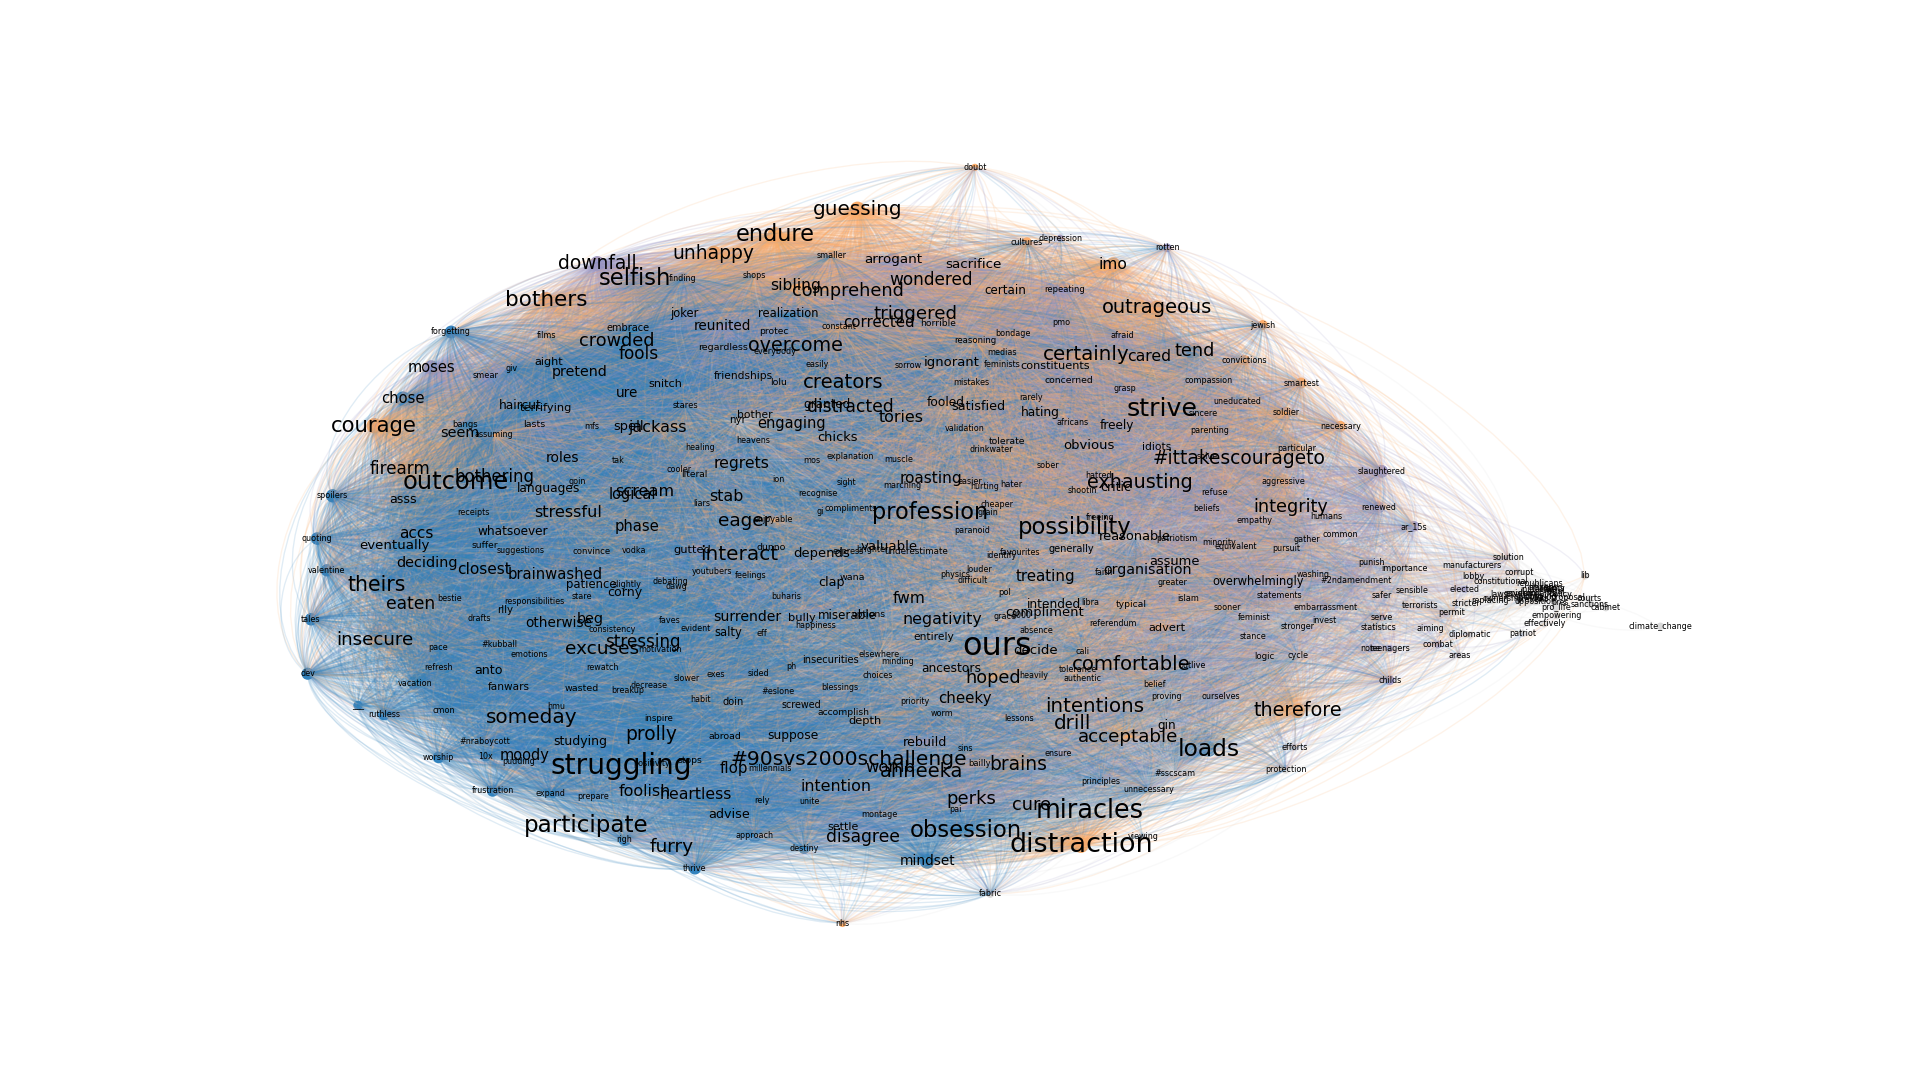
\includegraphics[width=\textwidth]{2Hop_ClimateChange_2018_02.png}
    \caption{The $2$-hop graph for ``climate\_change'' for the first word2vec model (trained on tweets from February 2018).}
    \label{fig:2hop_climate_change_FIRST}
\end{figure*}

\begin{figure*}
    \centering
    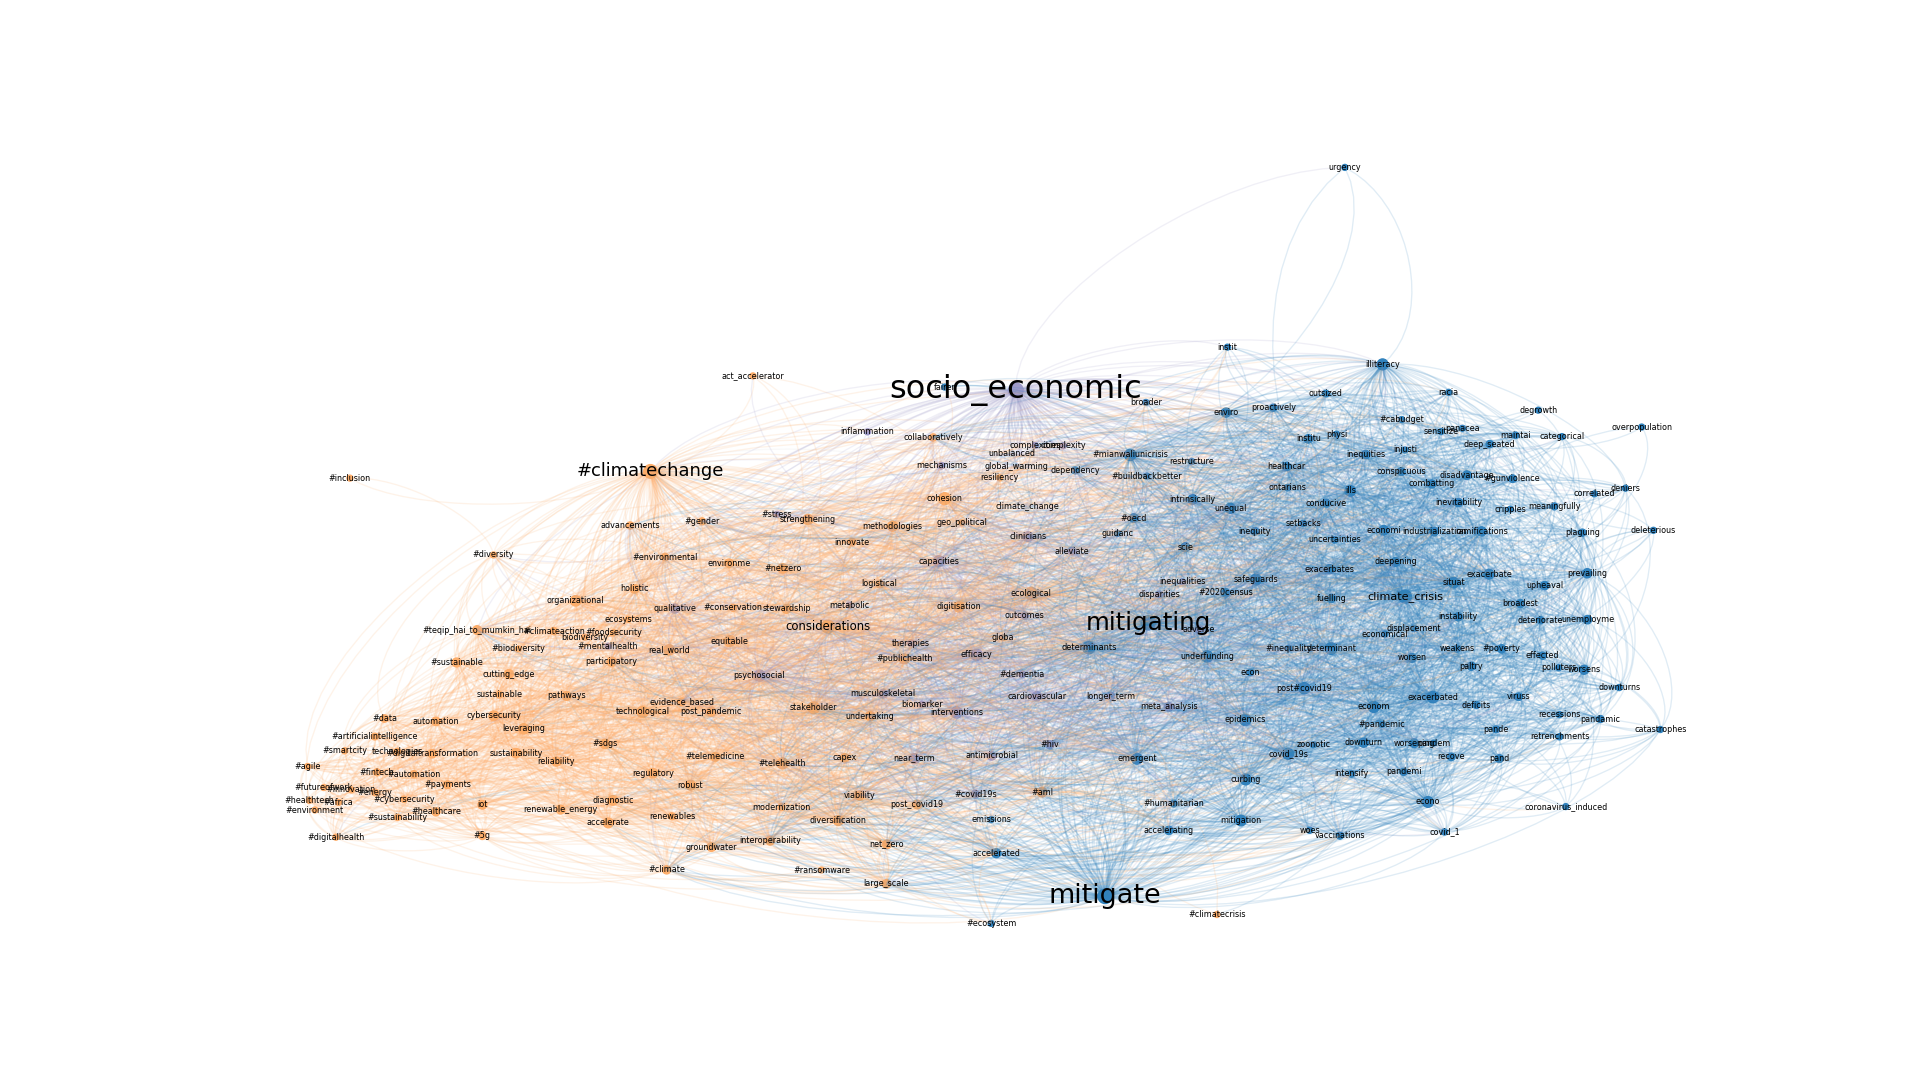
\includegraphics[width=\textwidth]{2Hop_ClimateChange_2020_06.png}
    \caption{The $2$-hop graph for ``climate\_change'' for the last word2vec model (trained on tweets from June 2020).}
    \label{fig:2hop_climate_change_LAST}
\end{figure*}

\subsection{Sentiment Analysis}
Using the sentiment classification model, we analyse the climate change sentiment of tweets. For each month, we take a 10\% random sample of all the tweets in the dataset, and then compute the climate change sentiment of each tweet (according to methodology presented in Section \ref{sec:methods}). Figure \ref{fig:sentiment_over_time} shows the average climate change sentiment per month, plotted on a $-1$ (negative) to $1$ (positive) scale. We see that the sentiment mostly hovers $0$, which suggests that most tweets are neutral. After all, this makes sense since Twitter is a general discussion platform, and the reality is that discussions about climate change are in the minority of all discussions. However, around February/March, 2020, we see an a fairly substantial increase in the climate change sentiment. This suggests not only an increase in climate changed related activity during that period of time, but also \textit{positive} discussion. Notice that this is the same time period for which we observed the spike in the cosine similarity graphs (Figure \ref{fig:similarity_skeptic}). On the other hand, we also see a dip in the climate change sentiment around June, 2019. Recall from Table \ref{tab:major_events} that this was around the time when the 46th G7 summit was \textit{supposed} to be held. Thus, this could suggest a response to the summit, where there was an increase in the activity of climate change skeptics.

\begin{figure}[!t]
    \centering
    \begin{tikzpicture}
        \pgfplotsset{compat=1.12}
            \begin{axis}[
                title={Average Sentiment of Tweets},
                align=center,
                date coordinates in=x,
                % xtick=data,
                xticklabel style=
            		{rotate=60, anchor=east, yshift=-10pt},
                xticklabel={\year.\month},
                date ZERO=2009-08-18,% <- improves precision!
                max space between ticks=100pt,
                try min ticks=10,
                legend pos=north west,
                ylabel={Average Sentiment},
                grid=major
            ]
            \addplot+ [thick, mark=none] table {\SentimentOverTime};
            \draw [color=eventColour,dashed, ultra thick] (2018-6-8,-1) -- (2018-6-8,1);
            \draw [color=eventColour,dashed, ultra thick] (2018-9-14,-1) -- (2018-9-14,1);
            \draw [color=eventColour,dashed, ultra thick] (2019-8-19,-1) -- (2019-8-19,1);
            \draw [color=eventColour,dashed, ultra thick] (2019-9-20,-1) -- (2019-9-20,1);
            \draw [color=eventColour,dashed, ultra thick] (2019-11-4,-1) -- (2019-11-4,1);
            \draw [color=eventColour,dashed, ultra thick] (2020-6-12,-1) -- (2020-6-12,1);
        \end{axis}
    \end{tikzpicture}
    \caption{The average climate change sentiment of a 10\% random sample per month, plotted on a $-1$ to $1$ scale. The score of a tweet is assigned as follows: $1$ if positive, $-1$ if negative, and $0$ if neutral.}
    \label{fig:sentiment_over_time}
\end{figure}

\section{Discussion}
Based on the results of the temporal, content, and sentiment analysis, we see how the climate change sentiment of Twitter users has been shifting to one that is more serious, polarized; it echos the dire situation, and the current state of the climate emergency. As shown in the Section \ref{sec:results}, there is a high emphasis on climate change on Twitter. We also see how discussions about climate change on Twitter have become more `severe', and that tweets are more likely to be of a positive sentiment (i.e. supporting climate change); that is, to be associated with the `great' or `good' aspects of climate issue---as opposed skepticism and climate change denial.

Further research is desired to investigate how misinformation on Twitter is targeted to affect the sentiment of users. This remains inconclusive

% Start references
\FloatBarrier
\clearpage
\printbibliography[]


\end{document}
